\documentclass{beamer}
\usetheme{Warsaw}
\usepackage{subcaption} % For subfigure captions
\usepackage[utf8]{inputenc}
\usepackage[T1]{fontenc}
\usepackage[french]{babel}

\title{Prediction of Oil Prices Turning Points with LPPL}
\author{B. Dufour J. Mourgues-Haroche T. Charbonnier A. Remiat}
\date{\today}

\begin{document}
\frame{\titlepage}

% Introduction
% \chapter{Introduction}
% \addcontentsline{toc}{chapter}{Introduction}

\begin{frame}
\frametitle{Introduction to financial bubbles modeling}
    Crude oil is crucial to the global economy, with price volatility causing major economic and political disruptions. Accurately predicting price turning points is essential for strategic reserves and investment. \\
    This paper presents an enhanced LPPL model, optimized via a multi-population genetic algorithm (MPGA), for improved forecasting accuracy.
    \begin{block}{Keywords of the study}
        \begin{itemize}
            \item {Financial bubbles detection}
            \item {Non-linear models estimation}
            \item {Heuristic \& Genetic algorithms}
        \end{itemize}
    \end{block}
\end{frame}

% Table des matières
%\tableofcontents
%\newpage

% --------------------------------------------------------------
% Chapitre 1
%\chapter{LPPL and Optimisation Algorithms}

% **************************************************************
% LPPL
%\section{LPPL}

\begin{frame}{Context of LPPL Models}
    \begin{itemize}
        \item LPPL models aim to describe speculative bubbles in financial markets.
        \item \textbf{Key Assumption:} A bubble exhibits super-exponential growth with log-periodic oscillations as it approaches a critical point.
        \item \textbf{Motivation:} To capture the interplay between rational traders and noise traders in destabilizing the market.
    \end{itemize}
    \begin{block}{Historical Use}
        \begin{itemize}
            \item Empirical validation on commodities and equity indices.
            \item Interesting extensions on currencies and cryptocurrencies
        \end{itemize}
    \end{block}
\end{frame}

\begin{frame}{Agent-Based Foundations of LPPL Models}
    \begin{block}{Traders interplay : The Ising model}
        Each trader’s position (\(s_i = +1\) for long, \(s_i = -1\) for short) is determined by:
        \[
        s_i = \text{sign}\left( \sum_{j \in N(i)} K s_j + \sigma \epsilon_i + G \right),
        \]
        where:
        \begin{itemize}
            \item \(N(i)\): Trader \(i\)’s network.
            \item \(K > 0\): Coupling strength (influence of peers).
            \item \(\sigma > 0\): Strength of idiosyncratic factors.
            \item \(\epsilon_i \sim N(0,1)\): Independent random shock.
            \item \(G\): Global influence.
        \end{itemize}
    \end{block}
\end{frame}

\begin{frame}
    \frametitle{Agent-Based Foundations of LPPL Models}
    {LPPL models are derived from agent-based interactions between:}
    \begin{itemize}
        \item \textbf{Noise traders:} Exhibit herding behavior, amplifying trends.
        \item \textbf{Rational traders:} Attempt to exploit mispricings but may fail to stabilize the market.
    \end{itemize}
    \begin{block}{Conditional Crash Probability}
        The conditional probability of a crash, \(h(t)\), given that the bubble has not yet burst, represents the likelihood of a sudden collective sell-off:
        \[
        h(t) = B (t_c - t)^{-b}, \quad b \in (0, 1).
        \]
        This describes the increasing risk of market makers failing to absorb shocks as \(t\) approaches \(t_c\).
    \end{block}
\end{frame}

% Slide 2: LPPL Equation
\begin{frame}{Log-Periodic Power Law Equation}
    \begin{block}{General LPPL Form}
        \[p(t) = A + B (T_c - t)^{\alpha} + C (T_c - t)^{\alpha} \cos \left(\omega \ln (T_c - t) + \phi\right)
        \]
        \begin{itemize}
            \item \(p(t)\): Asset price or market indicator.
            \item \(t_c\): Critical time (crash or turning point).
            \item \(A, B, C, \omega, \phi\): Other parameters to be estimated.
            \item \(\alpha\): Critical exponent (\(0 < \alpha < 1\)).
        \end{itemize}
    \end{block}
    {Interpretation}
        \begin{itemize}
            \item Feedback loops create instability, while oscillations arise from trader interactions.
            \item Explains market crashes as endogenous events, not purely external shocks.
        \end{itemize}
\end{frame}

\begin{frame}
\frametitle{Derivation of linear parameters}
\begin{itemize}
    \item Linear parameters can be directly derived using a least squares approach for given nonlinear parameters:
    \item Definitions:
    \[
    f_j = (T_c - t_j)^{\alpha}
    \quad \text{and} \quad
    g_j = (T_c - t_j)^{\alpha} \cos \left( \omega \ln(T_c - t_j) + \phi \right)
    \]
    \[
    \begin{bmatrix}
    A \\
    B \\
    C
    \end{bmatrix}
    =
    \left( \mathbf{V}^T \mathbf{V} \right)^{-1} \mathbf{V}^T \mathbf{Y}
    \]
    where:
    \[
    \mathbf{V} =
    \begin{bmatrix}
    1 & f_1 & g_1 \\
    1 & f_2 & g_2 \\
    \vdots & \vdots & \vdots \\
    1 & f_J & g_J
    \end{bmatrix},
    \quad
    \mathbf{Y} =
    \begin{bmatrix}
    y(1) \\
    y(2) \\
    \vdots \\
    y(J)
    \end{bmatrix}
    \]
\end{itemize}
\end{frame}

% **************************************************************
% Turning points validation
%\section{Turning points validation}

% Slide: Lomb Periodogram Analysis
\begin{frame}{Lomb Periodogram Analysis in LPPL Models}
    \begin{block}{Purpose of the Analysis}
        \begin{itemize}
            \item The Lomb periodogram is used to validate the turning points (\(t_c\)) predicted by the LPPL model.
            \item It checks if the frequency \(\frac{\omega}{2\pi}\) derived from the LPPL fits matches the frequency of the periodic oscillations near the critical time \(t_c\).
        \end{itemize}
    \end{block}
    \begin{block}{Why the Lomb Periodogram?}
        \begin{itemize}
            \item Handles \textbf{non-uniform time series}, common in financial data.
            \item Provides an \textbf{objective method} for identifying periodic components.
            \item Effective for detecting periodic oscillations in noisy environments.
        \end{itemize}
    \end{block}
\end{frame}

\begin{frame}
\frametitle{Lomb Periodogram Method}
    \begin{block}{Power Spectral Density}
        The power spectral density \( P(f) \) is computed for the frequency series using the formula:
        \small
        \[
        P(f) = \frac{1}{2\sigma^2} \left[
        \begin{aligned}
        & \frac{
        \left( \sum_{j=1}^J (x_j - \bar{x}) \cos \left( 2\pi f (t_j - \tau) \right) \right)^2
        }{
        \sum_{j=1}^J \cos^2 \left( 2\pi f (t_j - \tau) \right)
        } \\
        & + \frac{
        \left( \sum_{j=1}^J (x_j - \bar{x}) \sin \left( 2\pi f (t_j - \tau) \right) \right)^2
        }{
        \sum_{j=1}^J \sin^2 \left( 2\pi f (t_j - \tau) \right)
        }
        \end{aligned}
        \right]
        \]
        \raggedright
        Where :
        \begin{itemize}
            \item \( x_j = y_j - A - B (t_c - t_j)^a \)
            \item \( \bar{x} \) is the mean of \( x_j \)
            \item \( \sigma^2 \) is the variance of \( x_j \).
        \end{itemize}
    \end{block}
\end{frame}

\begin{frame}
\frametitle{Frequency Calculation in Lomb Periodogram}
    \begin{block}{Offset time}
        The time offset \( t \) is calculated as:
        \[
        t = \frac{1}{4\pi f} \arctan \left( \sum_{j=1}^J \sin(4\pi f t_j) \Big/ \sum_{j=1}^J \cos(4\pi f t_j) \right)
        \]
        \begin{itemize}
            \item With \(tj = ln(t_c - t)^a \)
        \end{itemize}
    \end{block}
    \begin{block}{Key Process}
        \begin{itemize}
            \item Invalid frequencies in \(P(f)\) are removed (e.g., values below a threshold or the most probable frequency).
            \item If no valid values remain, the predicted turning points are \textbf{rejected}.
            \item Otherwise, the frequency with the \textbf{maximum valid value} is used.
        \end{itemize}
    \end{block}
\end{frame}

\begin{frame}{Validation of Turning Points with Lomb Periodogram}
    \begin{block}{Validation Criteria}
        \begin{itemize}
            \item The frequency from the Lomb periodogram is compared to \(\frac{\omega}{2\pi}\) from MPGA.
            \item A turning point is valid if the difference between frequencies is less than \(0.3\).
        \end{itemize}
    \end{block}
    \begin{block}{Conclusion}
        \begin{itemize}
            \item Only turning points passing the Lomb periodogram test are \textbf{recorded as valid}.
            \item Ensures robustness in predicting critical times (\(t_c\)) in LPPL analysis.
        \end{itemize}
    \end{block}
\end{frame}

% **************************************************************
% Optimisation algorithms
%\section{Optimisation algorithms}

\begin{frame}{Why Heuristic Algorithms for LPPL?}
    \begin{block}{Non-Linear Nature of LPPL}
        \begin{itemize}
            \item The LPPL model is highly \textbf{non-linear}, with parameters like \(\omega\), \(t_c\), and \(m\) interacting in complex ways.
            \item Standard estimation methods (e.g., least squares, likelihood) fail to estimate the model.
        \end{itemize}
    \end{block}
    \begin{block}{Heuristic Algorithms}
        \begin{itemize}
            \item \textbf{Definition:} Algorithms inspired by natural processes or optimization heuristics to explore large and complex solution spaces.
            \item Designed to:
            \begin{itemize}
                \item Avoid local minima.
                \item Handle high-dimensional, non-linear models effectively.
            \end{itemize}
            \item Examples: Genetic algorithms, simulated annealing, particle swarm optimization.
        \end{itemize}
    \end{block}
\end{frame}

\begin{frame}
    \frametitle{Genetic Algorithms: Principles}
    \textbf{Key Concepts:}
        \begin{itemize}
            \item Inspired by \textbf{natural evolution} and genetic selection.
            \item Operates on a population of candidate solutions, evolving them through:
            \begin{itemize}
                \item \textbf{Selection:} Fittest individuals are chosen for reproduction.
                \item \textbf{Crossover:} Genetic material is combined to create offspring.
                \item \textbf{Mutation:} Small random changes introduce diversity.
            \end{itemize}
        \end{itemize}
    \begin{block}{Why GAs for LPPL?}
        \begin{itemize}
            \item Effectively searches non-linear, multi-dimensional parameter spaces.
            \item Balances \textbf{exploration} (diverse solutions) and \textbf{exploitation} (refining good solutions).
        \end{itemize}
    \end{block}
\end{frame}

\begin{frame}{Multi-Population Genetic Algorithm (MPGA)}
    \begin{block}{Principle of MPGA}
        \begin{itemize}
            \item MPGA extends standard genetic algorithms by introducing \textbf{multiple sub-populations}.
            \item Each sub-population evolves independently, avoiding premature convergence to local minima.
            \item Periodic \textbf{migration of individuals} between populations introduces diversity and improves global search.
        \end{itemize}
    \end{block}
    \begin{block}{Advantages for LPPL Estimation}
        \begin{itemize}
            \item \textbf{Avoids local minima:} Independent sub-populations explore different areas of the parameter space.
            \item \textbf{Improved convergence:} Migration ensures diversity and prevents stagnation.
            \item \textbf{Effective for LPPL:} Handles the complex, multi-modal structure of the LPPL model.
        \end{itemize}
    \end{block}
\end{frame}

\begin{frame}
\frametitle{MPGA Process}
    \begin{center}
        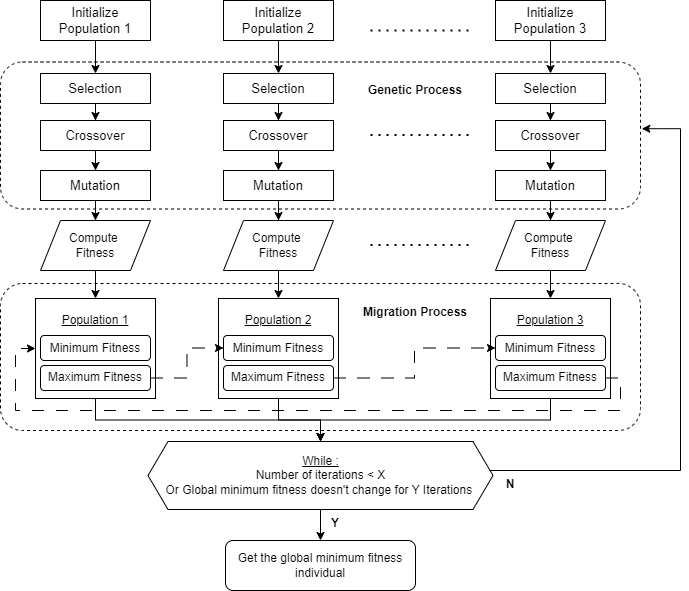
\includegraphics[scale=0.38]{pic/MPGA.drawio.png}
    \end{center}
\end{frame}

\begin{frame}{Particle Swarm Optimization (PSO)}
    \begin{block}{Principle of PSO}
        \begin{itemize}
            \item PSO is inspired by \textbf{social behavior of swarms} (e.g., birds).
            \item It optimizes a function by iteratively moving a population of particles (candidate solutions) through the search space.
            \item Each particle adjusts its position based on:
            \begin{itemize}
                \item \textbf{Personal Best (\(p_i\)):} Best solution it has found so far.
                \item \textbf{Global Best (\(g\)):} Best solution found in the entire swarm.
            \end{itemize}
        \end{itemize}
    \end{block}
    \begin{block}{PSO Algorithm Steps}
        \begin{enumerate}
            \item Initialize particles with random positions and velocities.
            \item Evaluate the fitness of each particle.
            \item Update velocities and positions:
            \[
            v_{i}(t+1) = w v_{i}(t) + c_1 r_1 (p_i - x_i) + c_2 r_2 (g - x_i)
            \]
            \[
            x_{i}(t+1) = x_{i}(t) + v_{i}(t+1)
            \]
        \end{enumerate}
    \end{block}
\end{frame}

\begin{frame}{Simulated Annealing (SA)}
    \begin{block}{Principle of SA}
        \begin{itemize}
            \item Simulated Annealing (SA) is inspired by the \textbf{annealing process} in metallurgy : Material is heated and slowly cooled to remove defects and reach a stable structure.

            \item SA mimics this by exploring the search space and accepting worse solutions to escape local minima.
        \end{itemize}
    \end{block}
    \begin{block}{SA Algorithm Steps}
        \begin{enumerate}
            \item Start with an initial solution and a high "temperature" \(T\).
            \item Generate a new candidate by making a small random change.
            \item Evaluate the fitness of the new solution:
            \begin{itemize}
                \item If better, accept it, else accept it with probability:
                \[
                P = \exp\left(-\frac{\Delta E}{T}\right),
                \]
                where \(\Delta E\) is the fitness difference.
            \end{itemize}
        \end{enumerate}
    \end{block}
\end{frame}

\begin{frame}
\frametitle{Turning points prediction in practice}
    \begin{center}
        \includegraphics[scale=0.4]{pic/processLPPL.png}
    \end{center}
\end{frame}

\begin{frame}
\frametitle{Framework Organization}
    \begin{center}
        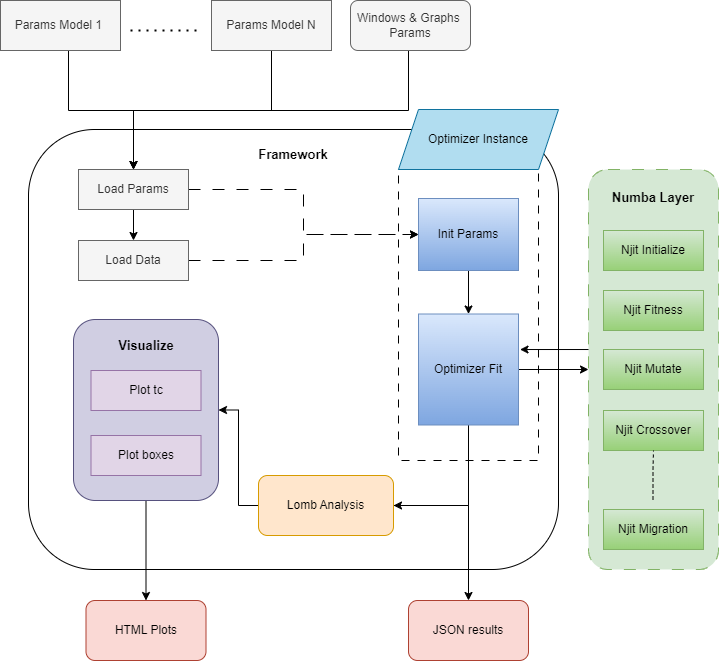
\includegraphics[scale=0.33]{pic/Framework.png}
    \end{center}
\end{frame}

\begin{frame}[h!]
    \centering
    \begin{minipage}[b]{0.45\textwidth}
        \centering
        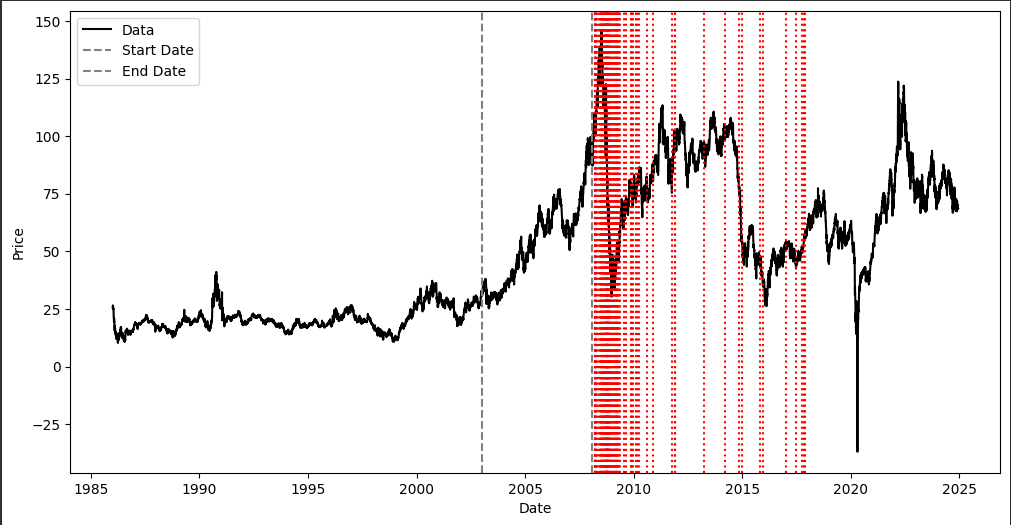
\includegraphics[width=\textwidth]{pic/daily/before_mpga.png}
        \captionof{subfigure}{Graph 1}
    \end{minipage}
    \hfill
    \begin{minipage}[b]{0.45\textwidth}
        \centering
        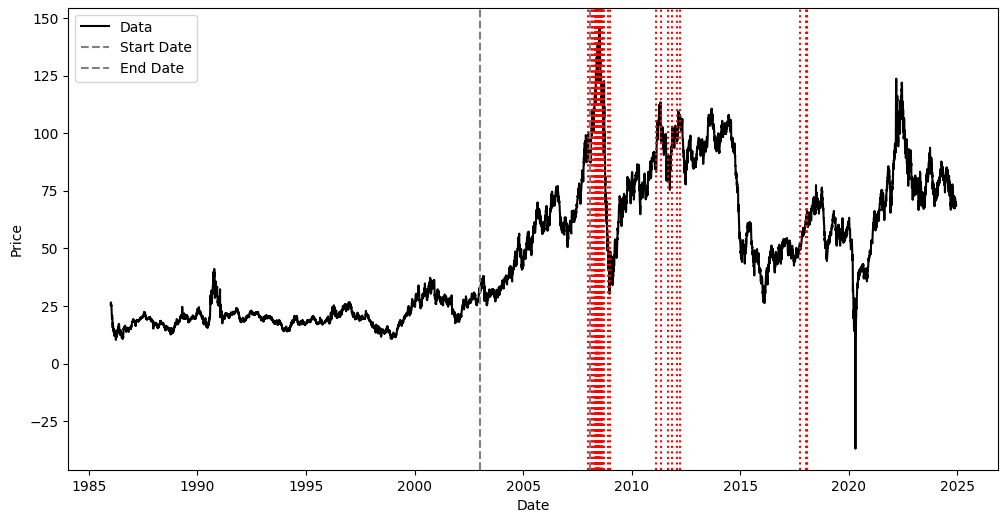
\includegraphics[width=\textwidth]{pic/daily/before_PSO.png}
        \captionof{subfigure}{Graph 2}
    \end{minipage}

    \vspace{0.5cm} % Vertical space between the rows (optional)

    \begin{minipage}[b]{0.45\textwidth}
        \centering
        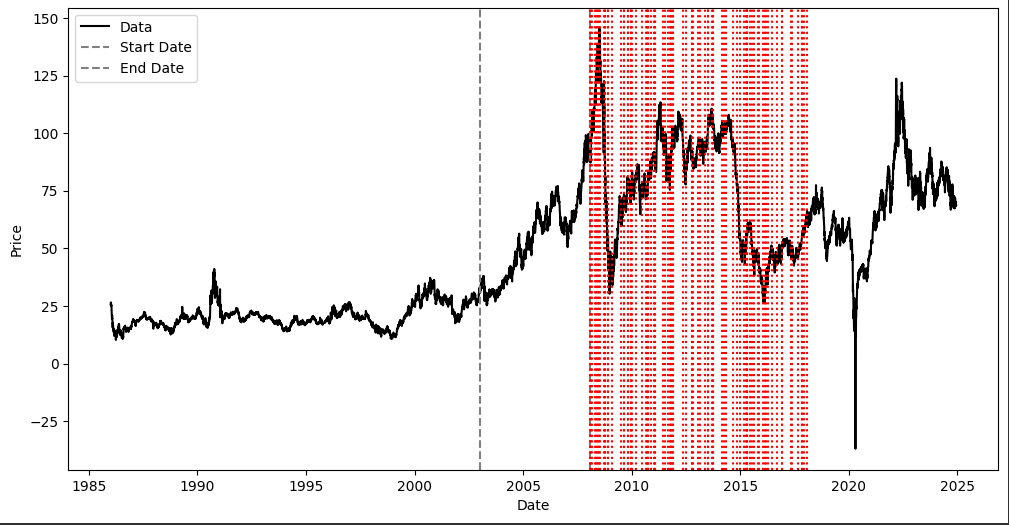
\includegraphics[width=\textwidth]{pic/daily/before_sga.png}
        \captionof{subfigure}{Graph 3}
    \end{minipage}
    \hfill
    \begin{minipage}[b]{0.45\textwidth}
        \centering
        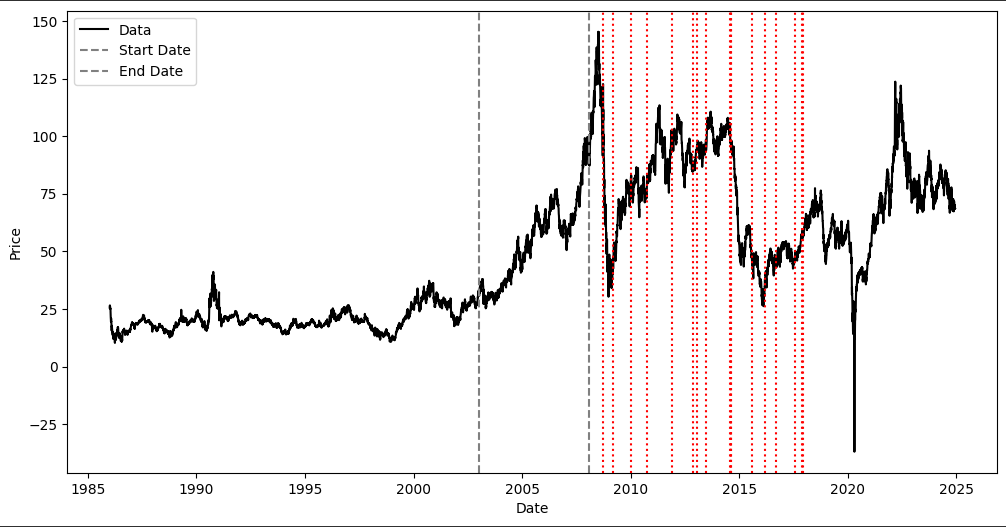
\includegraphics[width=\textwidth]{pic/daily/before_sa.png}
        \captionof{subfigure}{Graph 4}
    \end{minipage}

    \caption{Comparison of LPPLS predictions 04-2003 / 01-2008}
\end{frame}

\begin{frame}{Comparison of Prediction Results (daily)}
    \begin{center}
        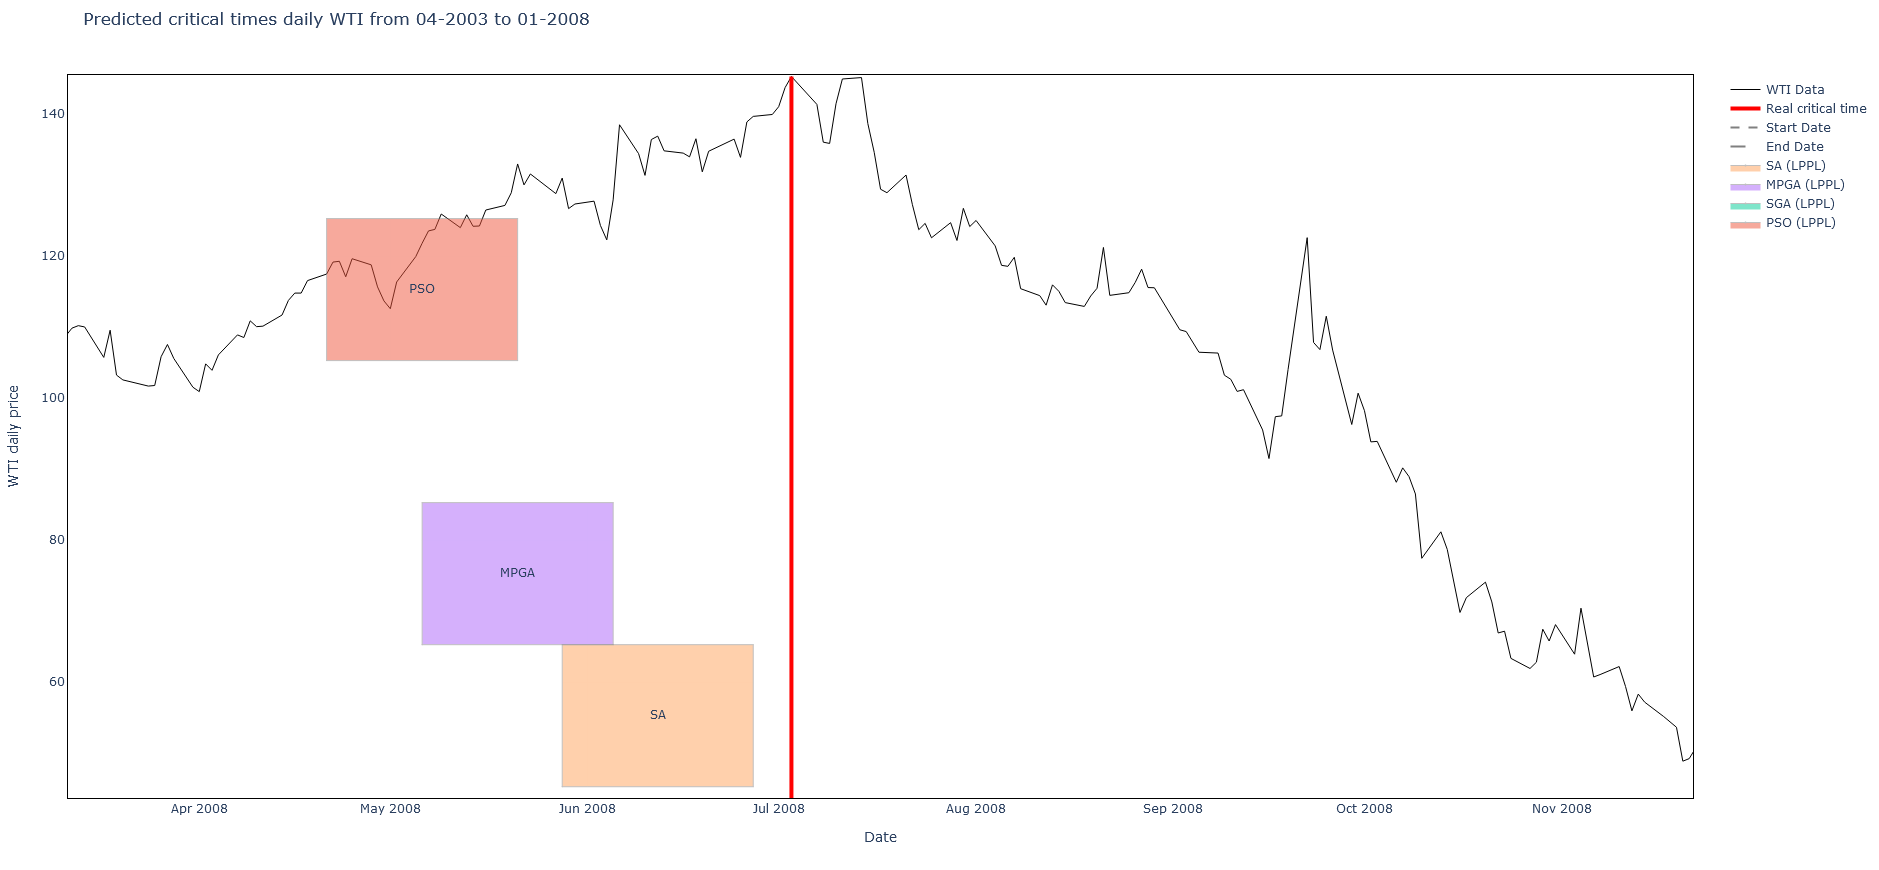
\includegraphics[width=\textwidth]{plot_overlead/daily_WTI_1.png}
    \end{center}
\end{frame}

\begin{frame}{Comparison of Prediction Results (daily)}
    \begin{center}
        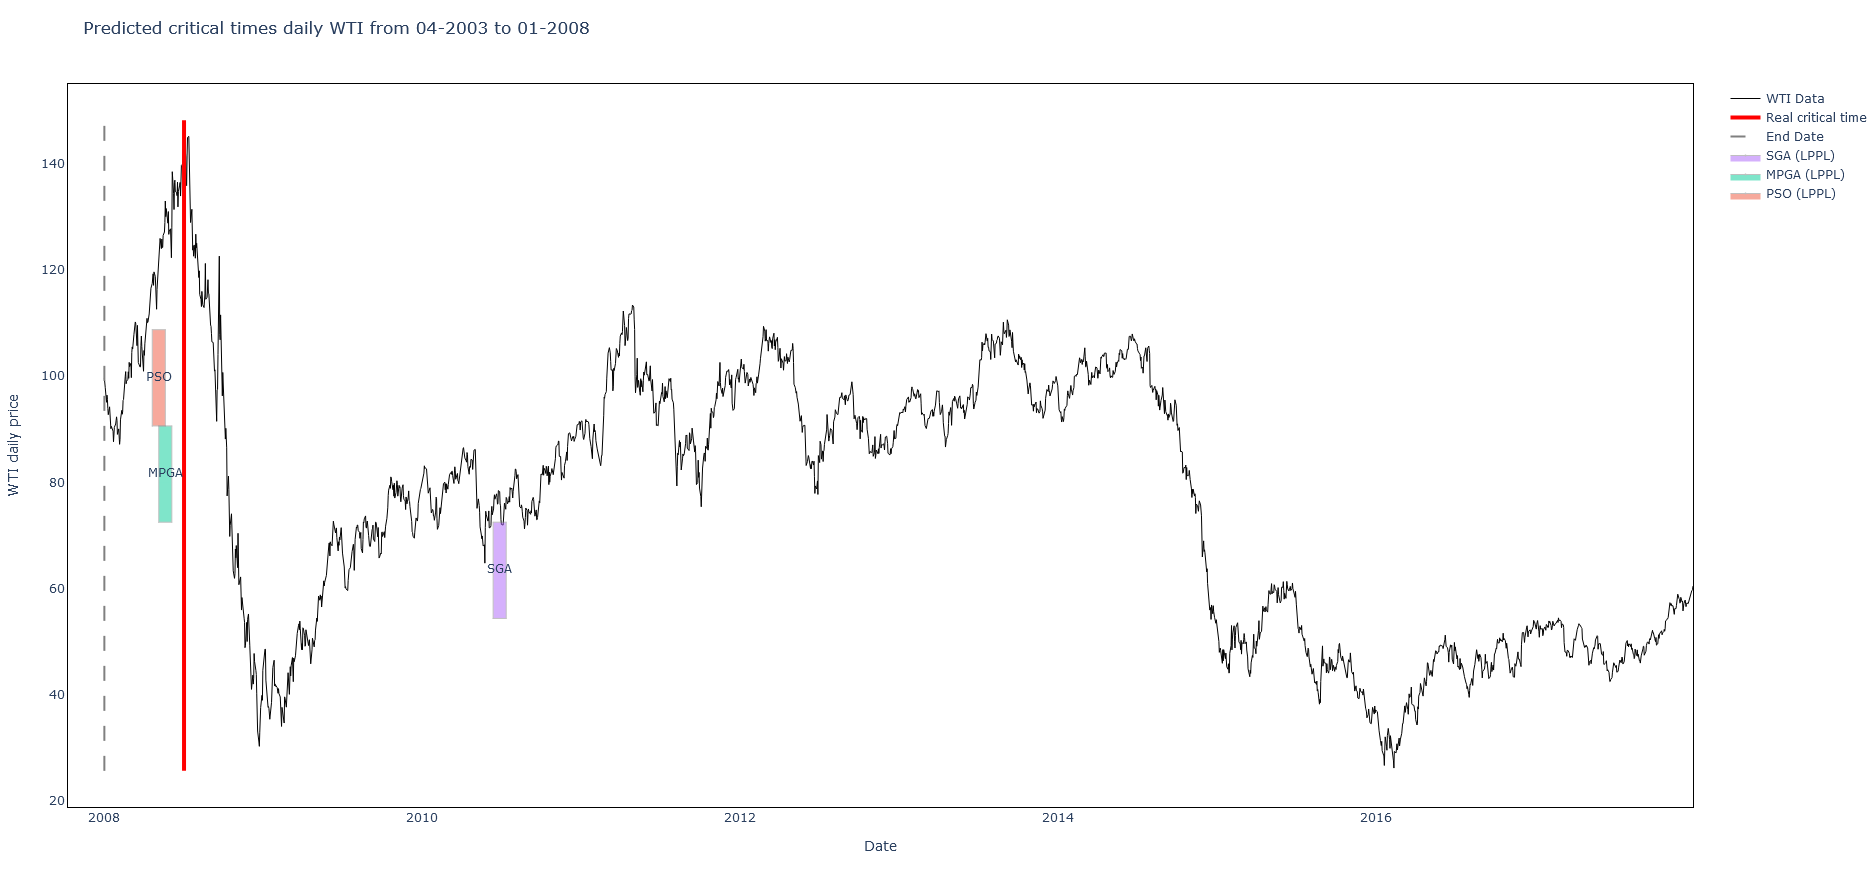
\includegraphics[width=\textwidth]{plot_overlead/daily_WTI_1_all_price.png}
    \end{center}
\end{frame}

\begin{frame}{Comparison of Prediction Results (daily)}
    \begin{center}
        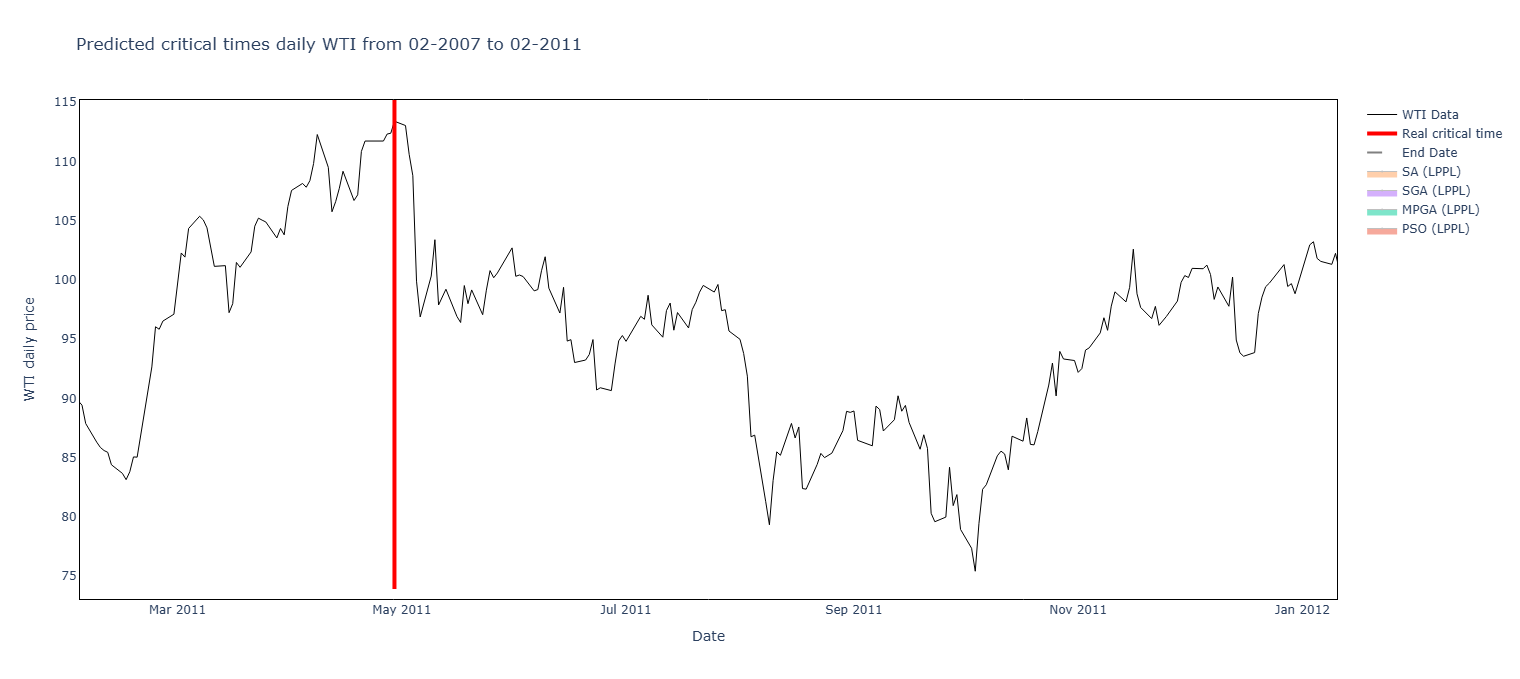
\includegraphics[width=\textwidth]{plot_overlead/daily_WTI_2.png}
    \end{center}
\end{frame}

\begin{frame}{Comparison of Prediction Results (daily)}
    \begin{center}
        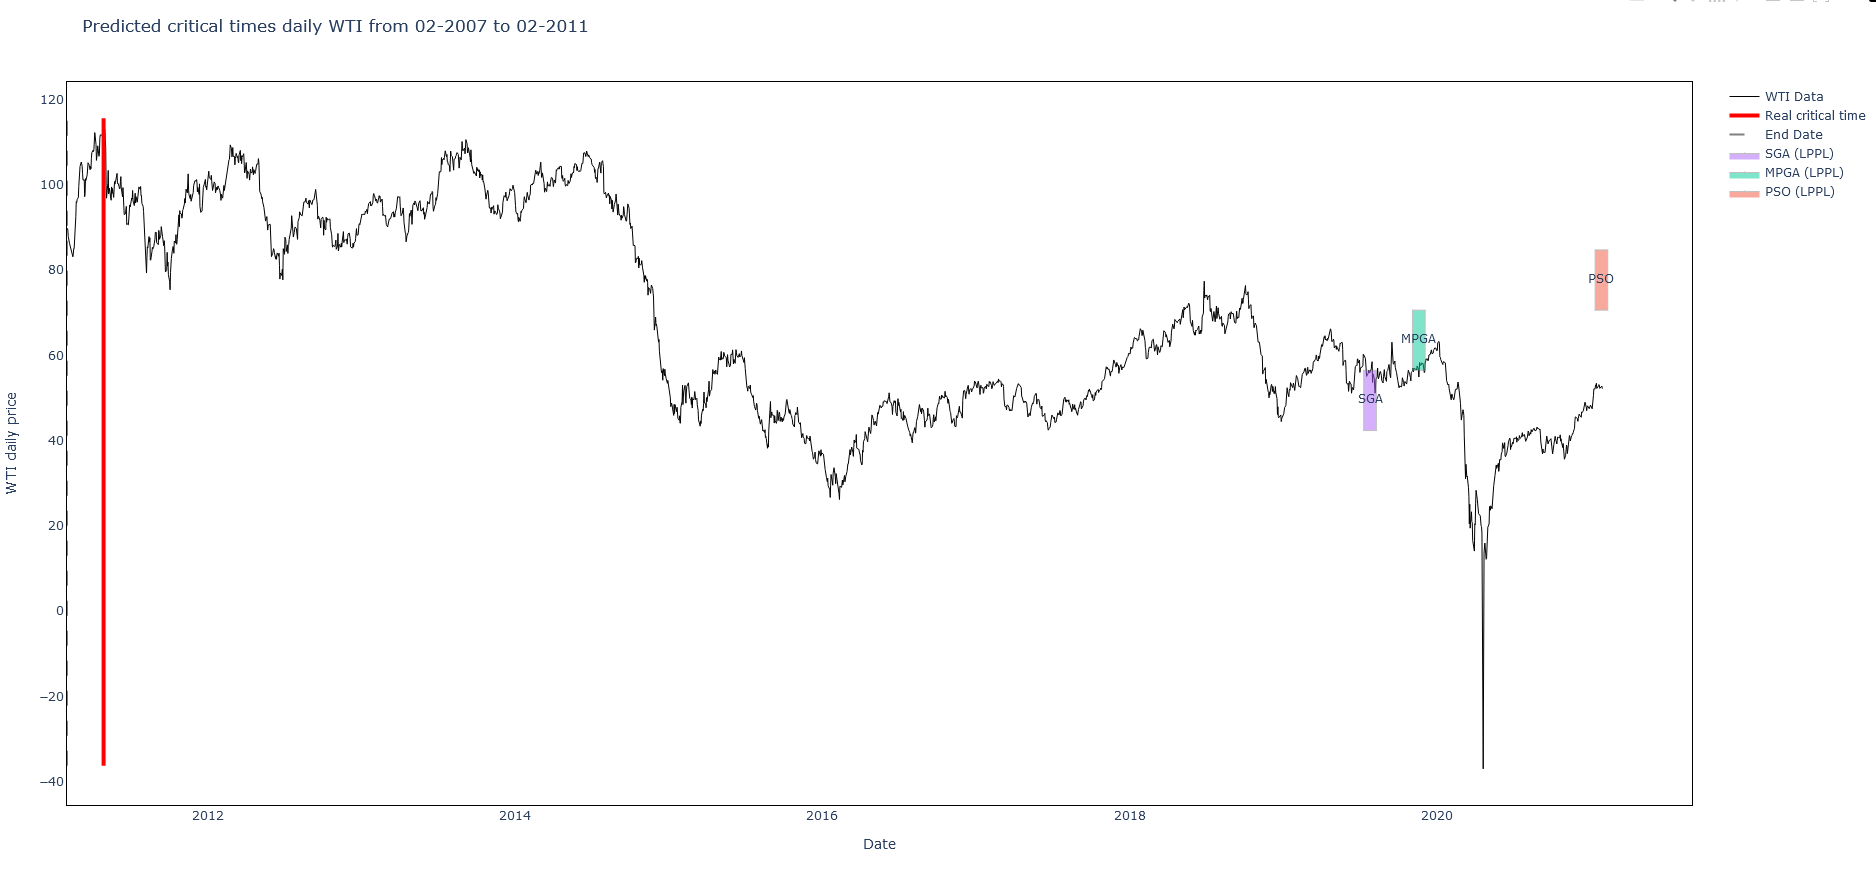
\includegraphics[width=\textwidth]{plot_overlead/daily_WTI_2_all_price.png}
    \end{center}
\end{frame}

\begin{frame}{Comparison of Prediction Results (daily)}
    \begin{center}
        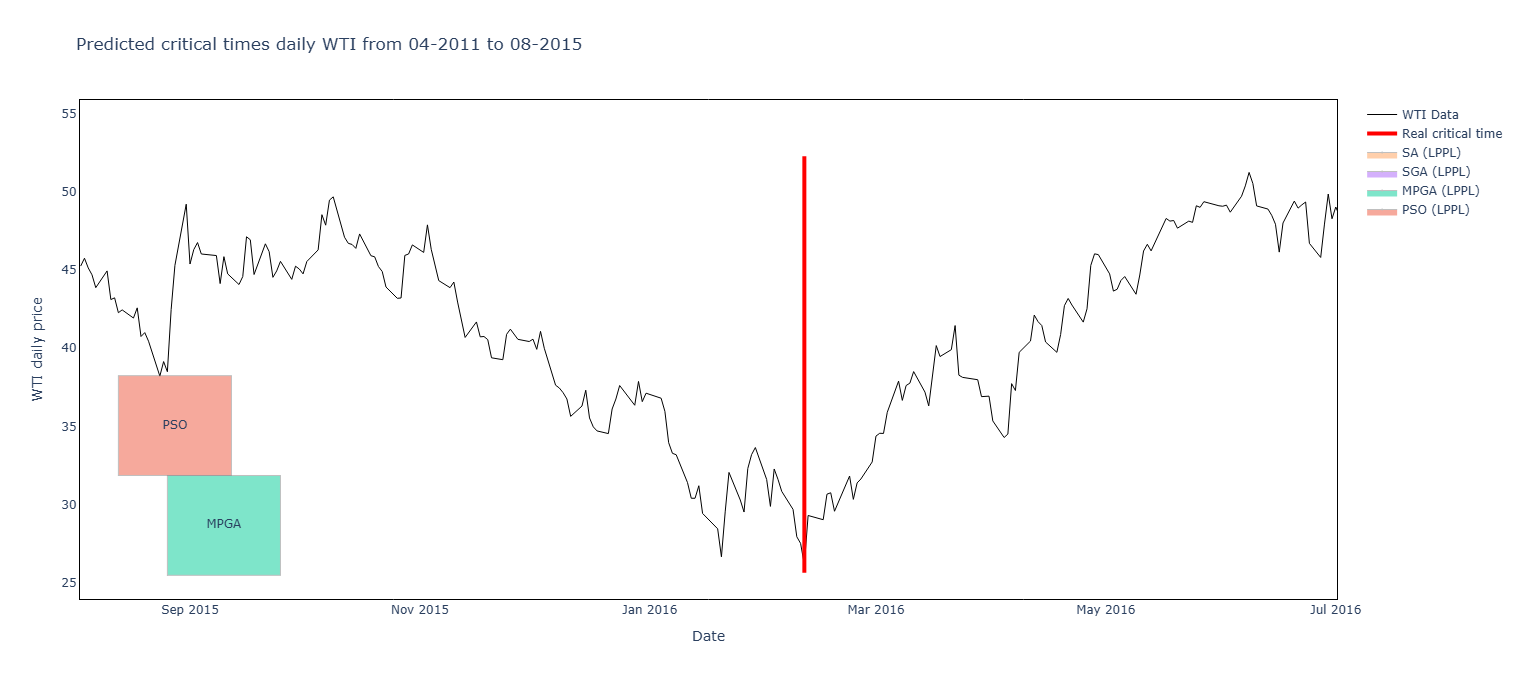
\includegraphics[width=\textwidth]{plot_overlead/daily_WTI_3.png}
    \end{center}
\end{frame}

\begin{frame}{Comparison of Prediction Results (daily)}
    \begin{center}
        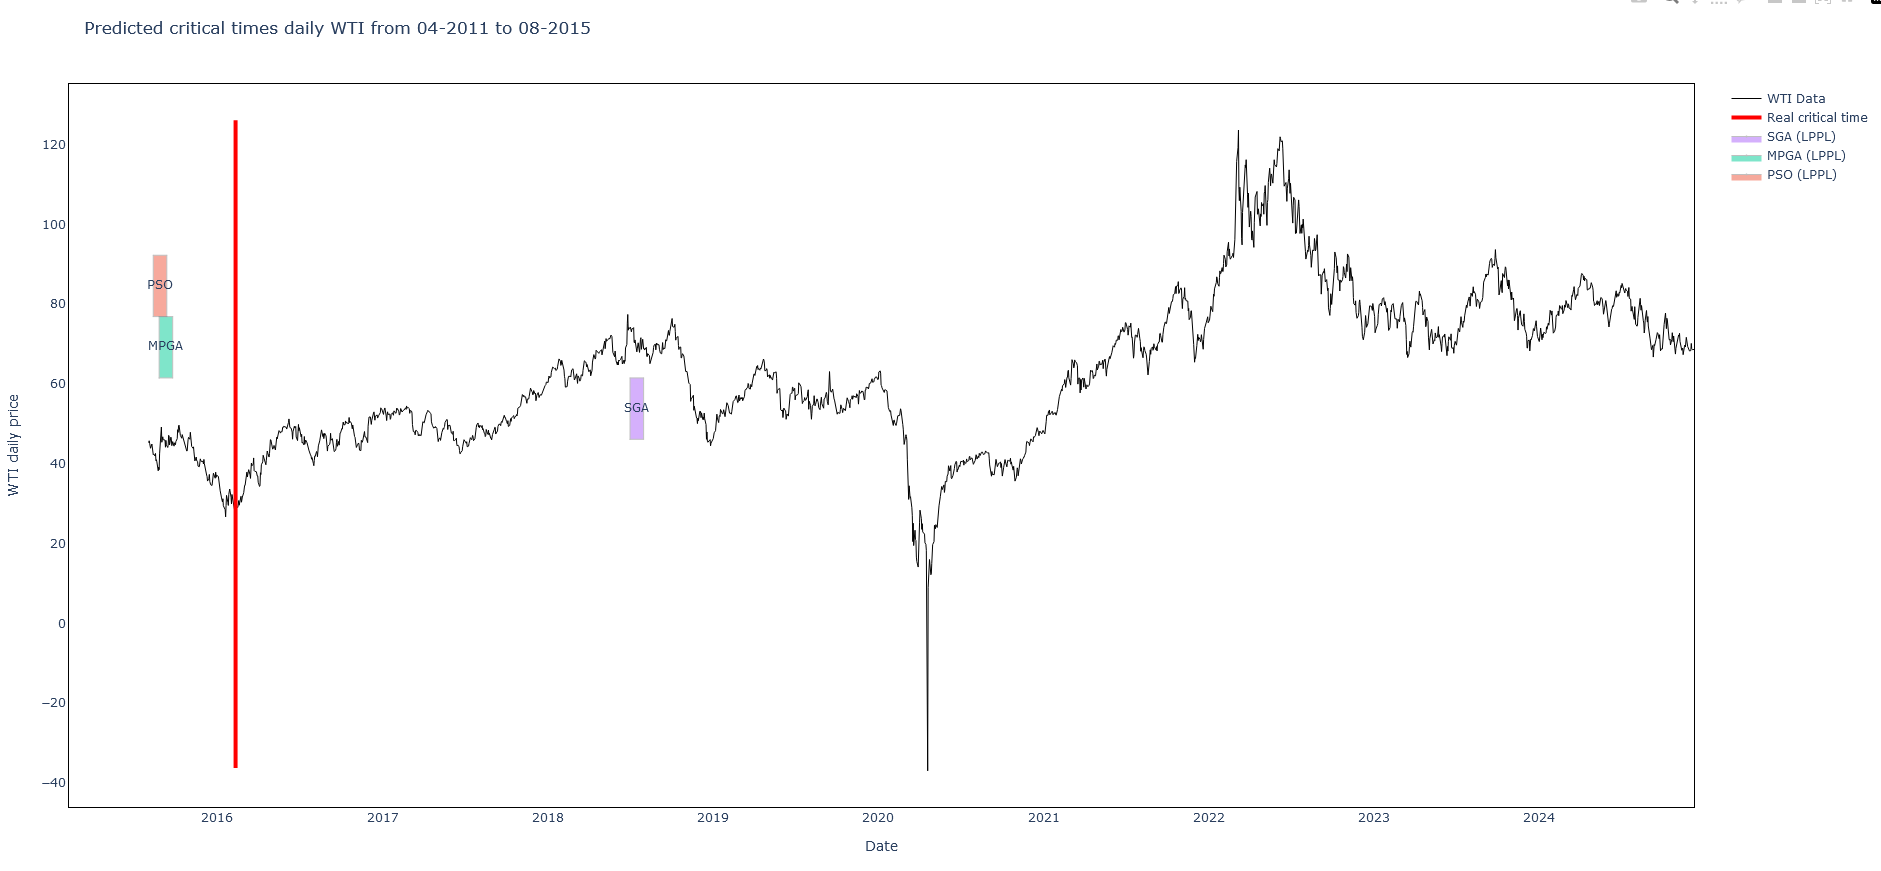
\includegraphics[width=\textwidth]{plot_overlead/daily_WTI_3_all_price.png}
    \end{center}
\end{frame}

\begin{frame}{Comparison of Prediction Results (weekly)}
    \begin{center}
        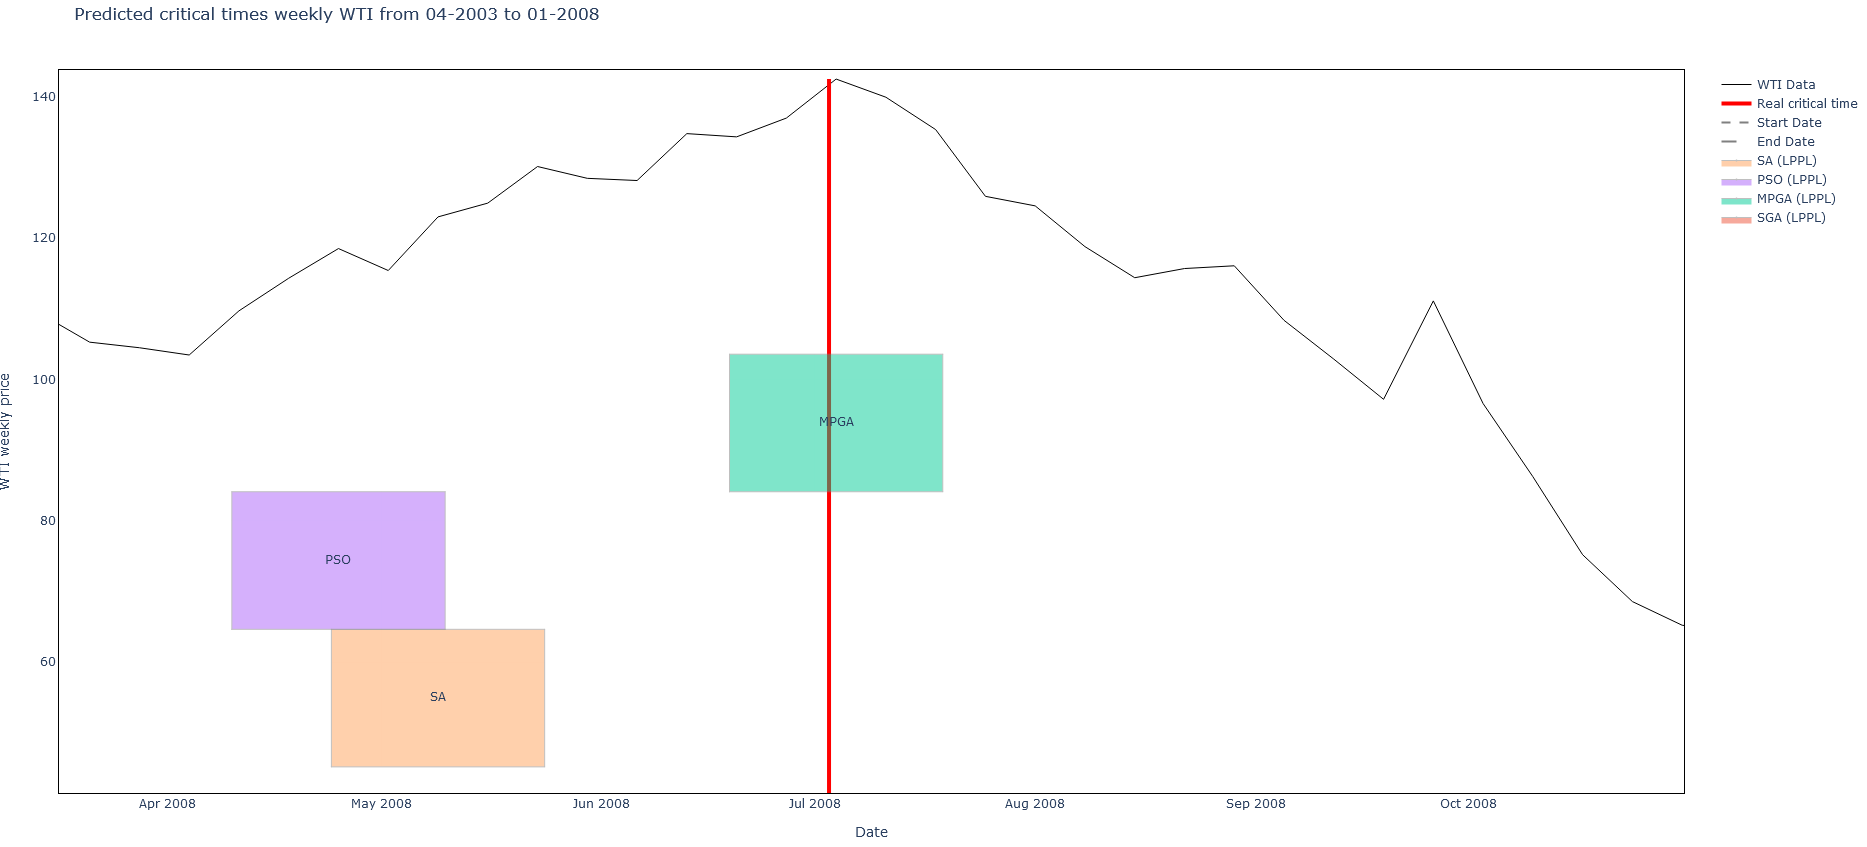
\includegraphics[width=\textwidth]{plot_overlead/weekly_WTI_1.png}
    \end{center}
\end{frame}

\begin{frame}{Comparison of Prediction Results (weekly)}
    \begin{center}
        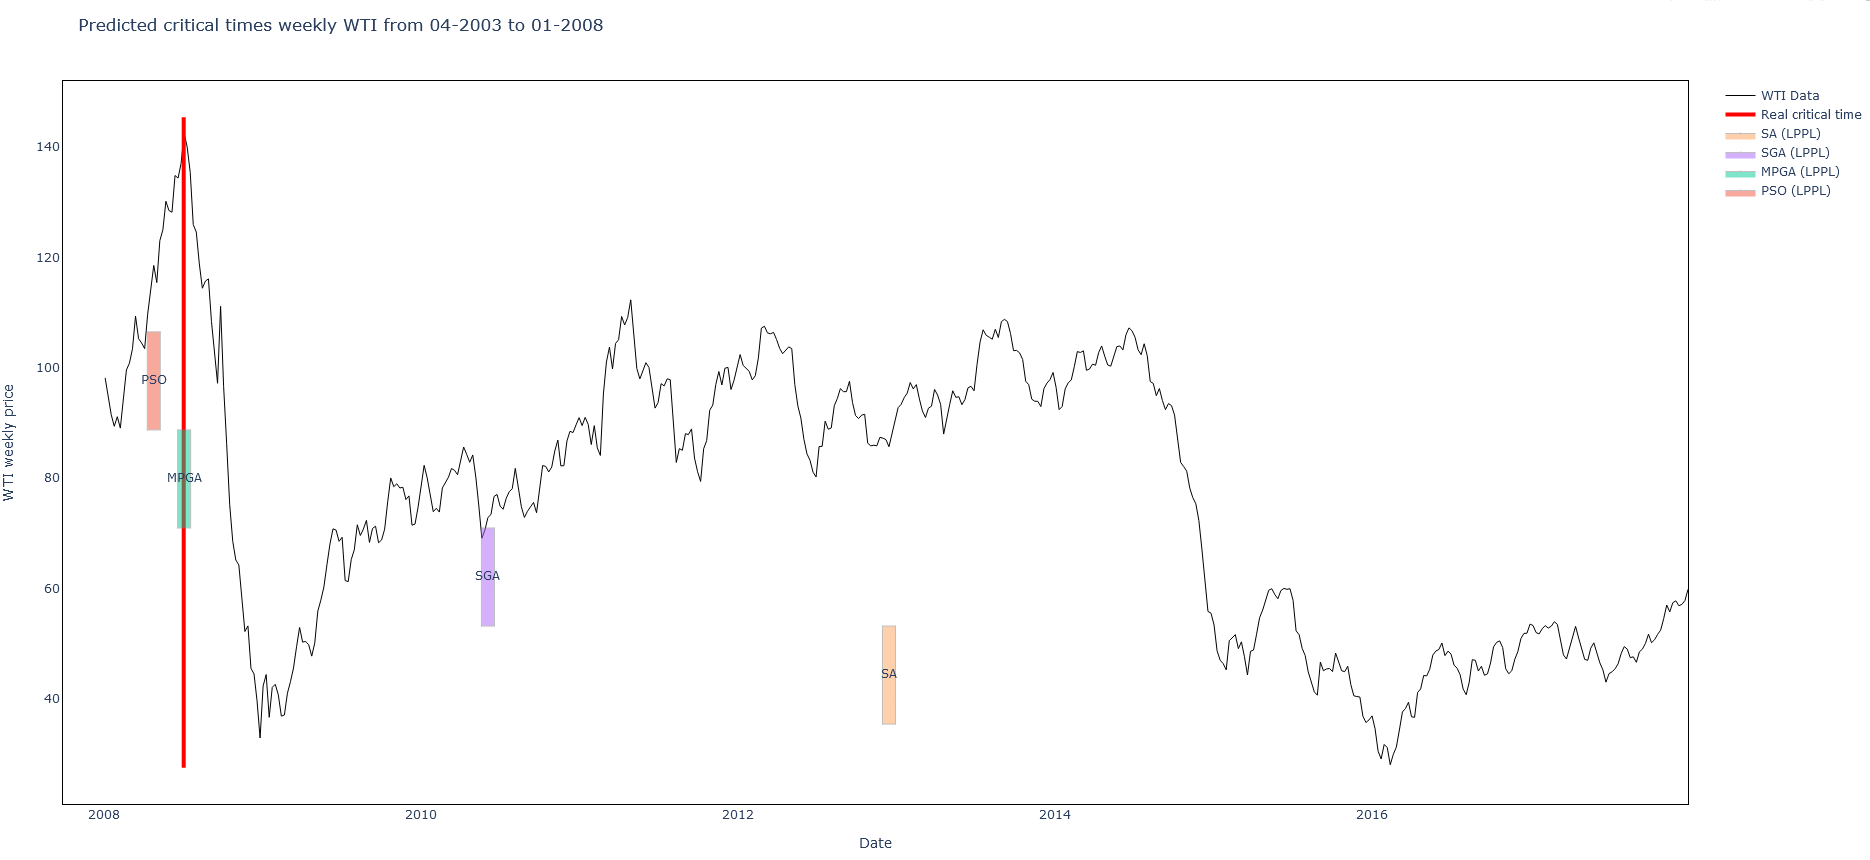
\includegraphics[width=\textwidth]{plot_overlead/weekly_WTI_1_all_price.png}
    \end{center}
\end{frame}

\begin{frame}{Comparison of Prediction Results (weekly)}
    \begin{center}
        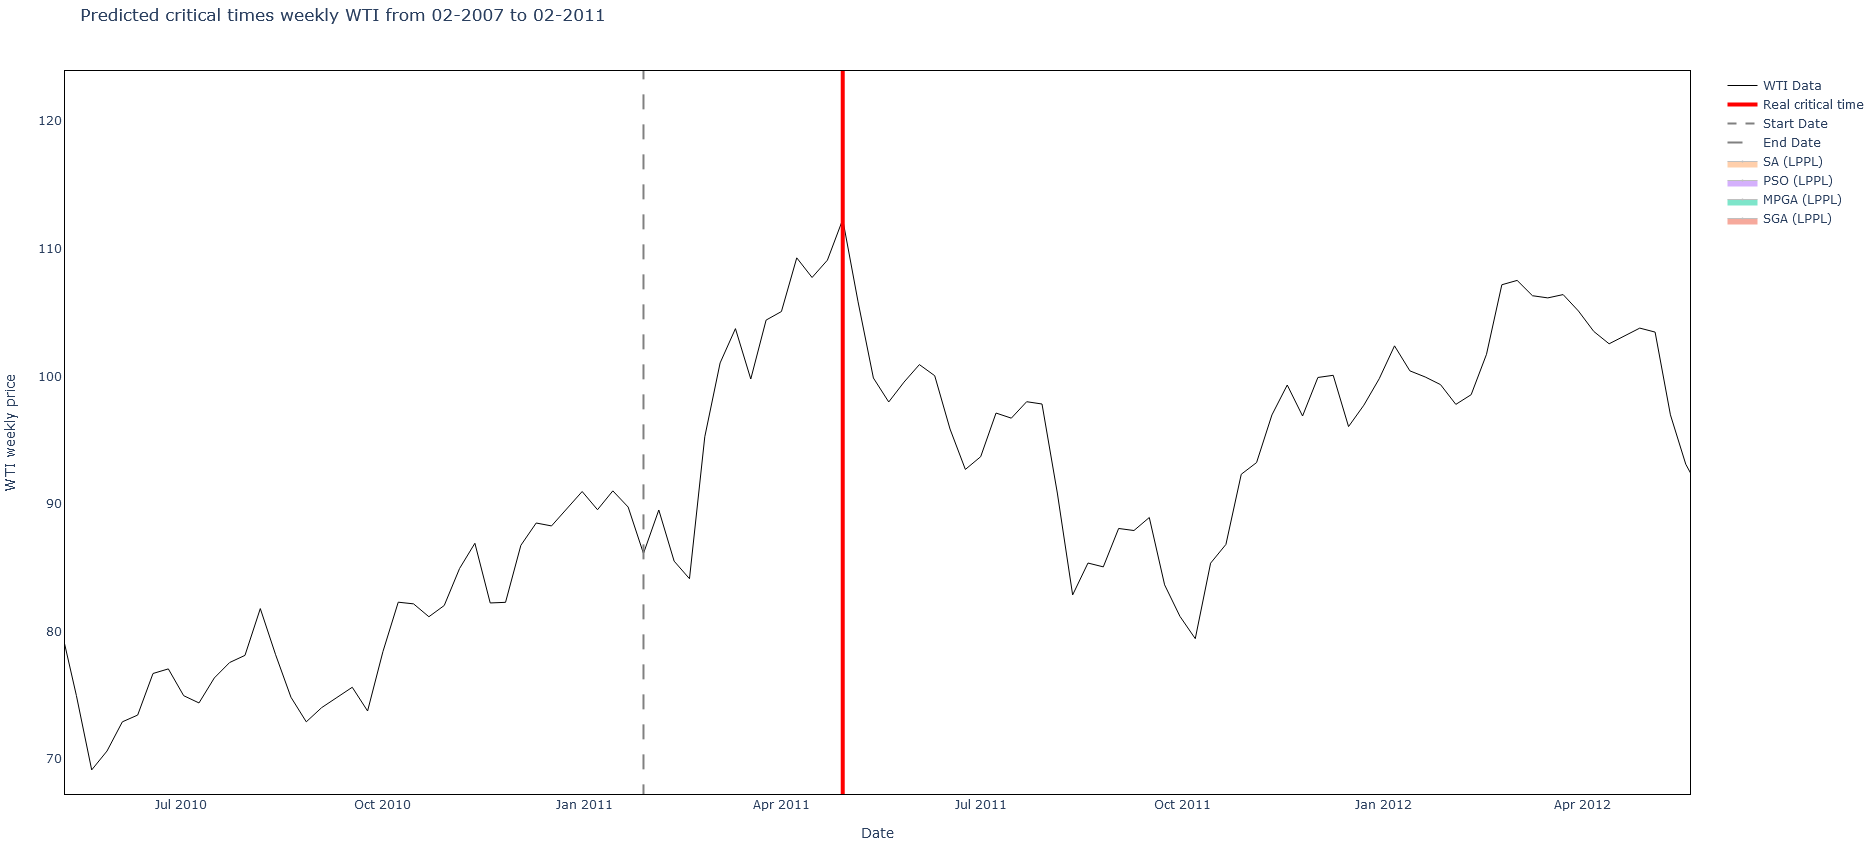
\includegraphics[width=\textwidth]{plot_overlead/weekly_WTI_2.png}
    \end{center}
\end{frame}

\begin{frame}{Comparison of Prediction Results (weekly)}
    \begin{center}
        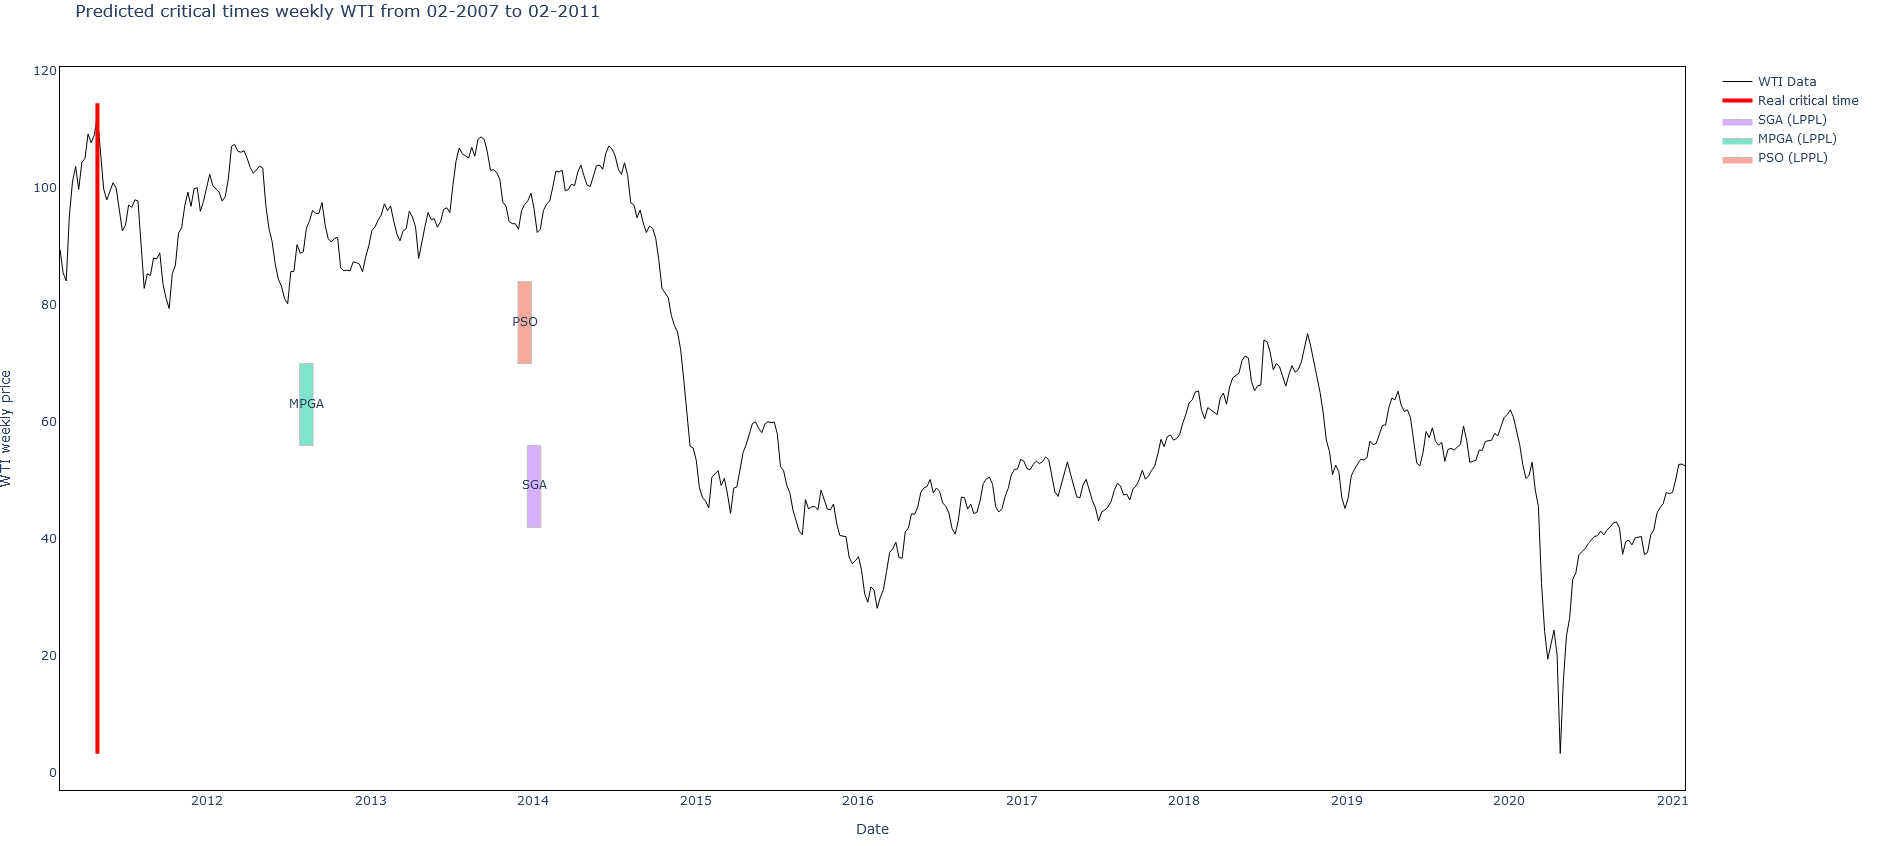
\includegraphics[width=\textwidth]{plot_overlead/weekly_WTI_2_all_price.png}
    \end{center}
\end{frame}

\begin{frame}{Comparison of Prediction Results (weekly)}
    \begin{center}
        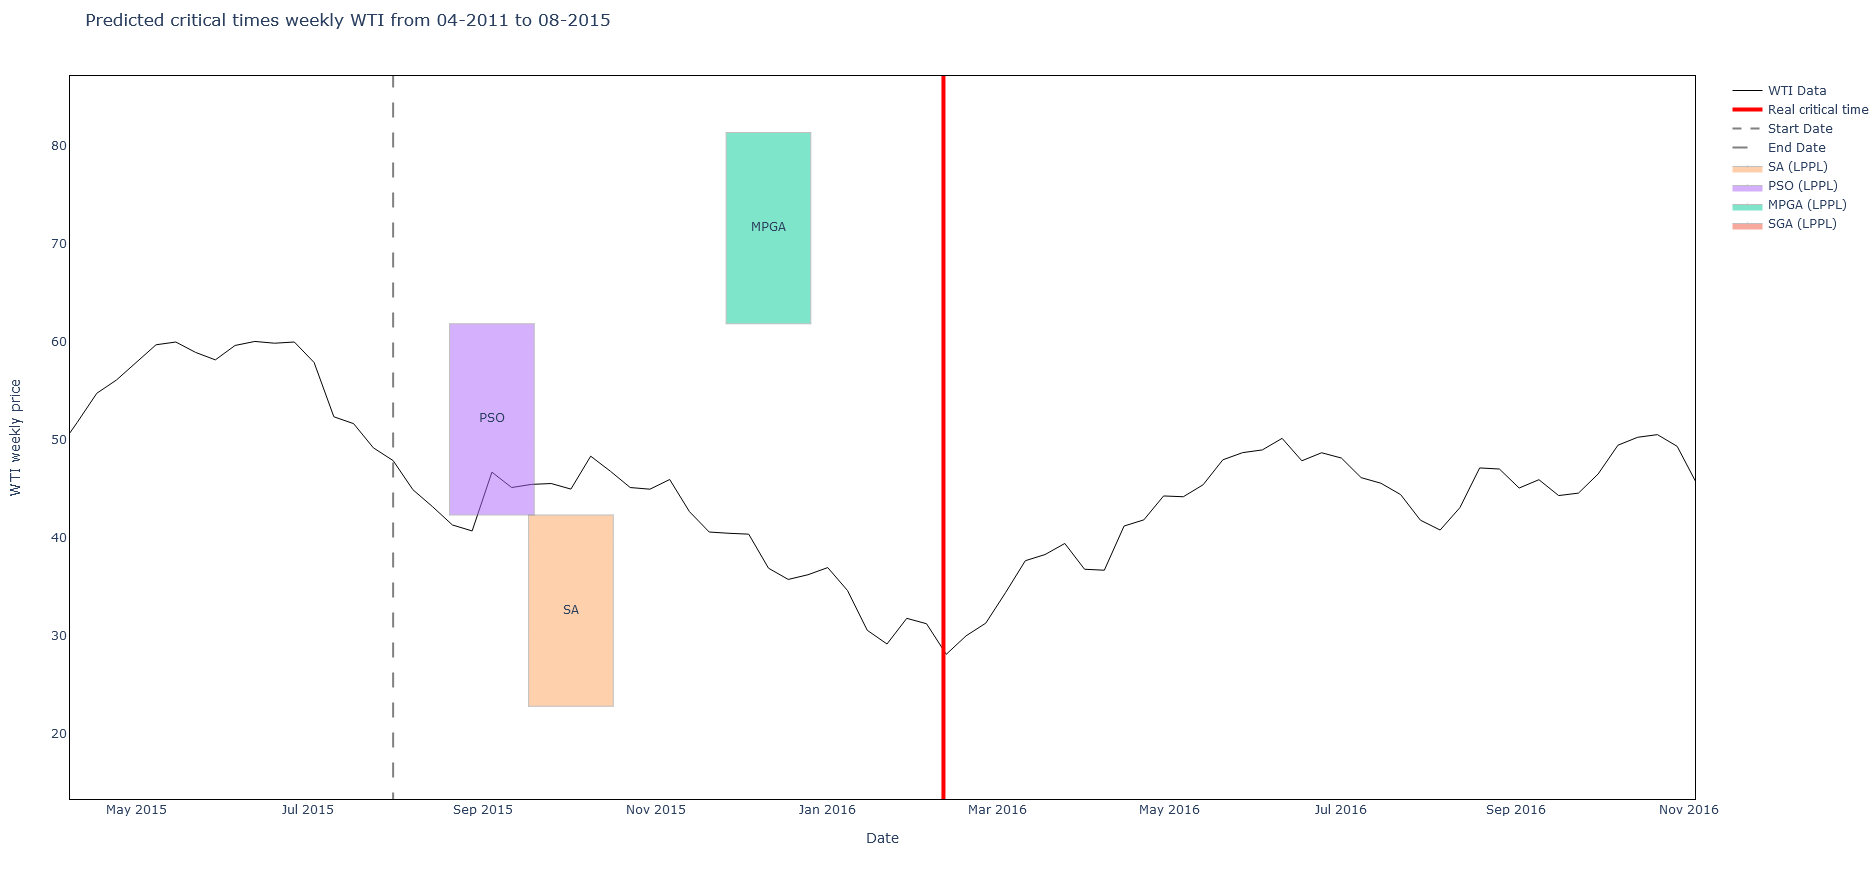
\includegraphics[width=\textwidth]{plot_overlead/weekly_WTI_3.png}
    \end{center}
\end{frame}

\begin{frame}{Comparison of Prediction Results (weekly)}
    \begin{center}
        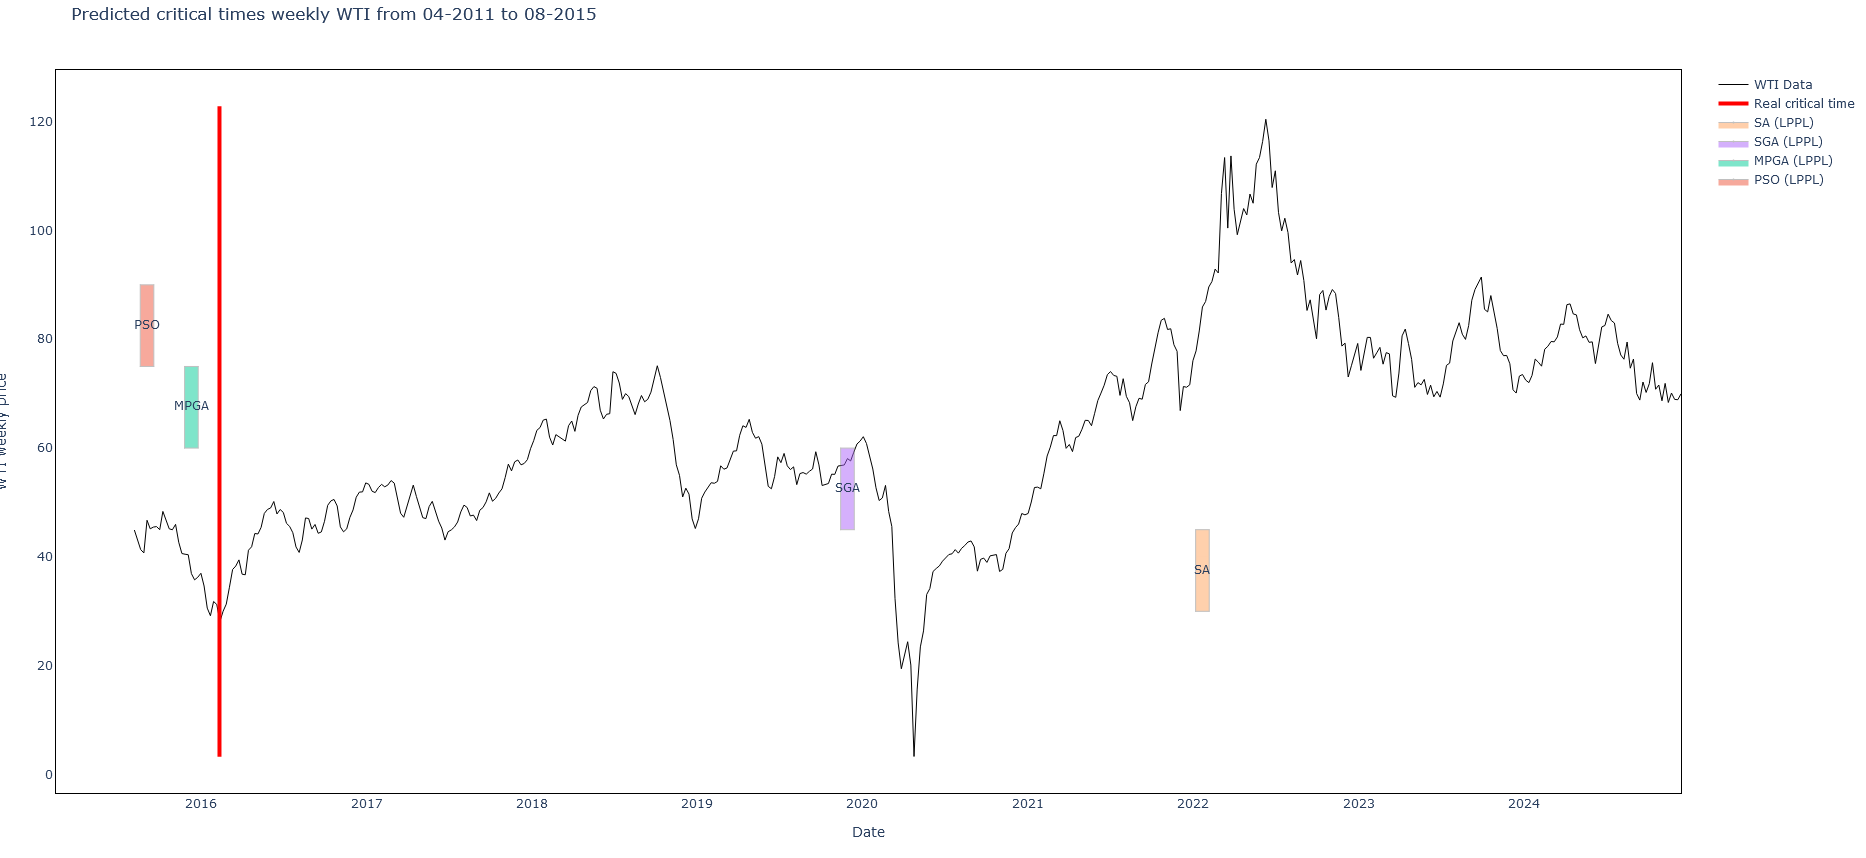
\includegraphics[width=\textwidth]{plot_overlead/weekly_WTI_3_all_price.png}
    \end{center}
\end{frame}

\begin{frame}{Comparison of Prediction Results}
\begin{table}[ht]
\centering
\caption{Comparison of prediction results of different heuristic algorithms.}
\resizebox{\textwidth}{!}{%
\begin{tabular}{|l|c|c|c|}
\hline
\textbf{Optimization Method} & \textbf{Turning Point 1} & \textbf{Turning Point 2} & \textbf{Turning Point 3} \\ \hline
Historical Turning Point     & \textbf{2008/07/03}      & \textbf{2011/04/29}      & \textbf{2016/02/11}      \\ \hline
30 days optimized by MPGA    & True (2008/06/29–2008/07/29) & True (2011/04/06–2011/05/06) & True (2016/02/10–2016/03/11) \\ \hline
4 weeks optimized by MPGA    & True (2008/06/20–2008/07/18) & True (2011/04/15–2011/05/13) & True (2016/01/15–2016/02/12) \\ \hline
30 days optimized by SGA     & True (2008/06/26–2008/07/26) & False (2011/09/04–2011/10/04) & False (2016/02/27–2016/03/28) \\ \hline
4 weeks optimized by SGA     & False (2008/07/11–2008/08/08) & False (2011/05/20–2011/06/17) & True (2016/02/05–2016/03/04) \\ \hline
30 days optimized by SA      & False (2008/06/26–2008/07/26) & False (2011/04/08–2011/05/08) & False (2016/02/19–2016/03/20) \\ \hline
4 weeks optimized by SA      & False (2008/06/27–2008/07/25) & False (2011/07/29–2011/08/26) & False (2016/01/15–2016/02/12) \\ \hline
30 days optimized by PSO     & False (2008/08/24–2008/09/23) & False (2011/06/17–2011/07/15) & False (2015/10/12–2015/11/11) \\ \hline
4 weeks optimized by PSO     & False (2008/07/11–2008/08/08) & False (2011/06/17–2011/07/15) & False (2015/08/21–2015/09/18) \\ \hline
\end{tabular}%
}
\end{table}
\end{frame}

\begin{frame}{MCMC Algorithm}
    \frametitle{Extensions : MCMC Algorithm}
    \begin{block}{Steps in LPPL Estimation with Metropolis-Hastings}
        \begin{itemize}
            \item \textbf{Define the Likelihood Function:}
                  \[
                  P(\text{Data} | \theta) = \exp\left(-\frac{1}{2} \sum_{i=1}^N \left[\ln p(t_i) - f(t_i; \theta)\right]^2\right)
                  \]
            \item \textbf{Set Priors:} Define prior distributions for \(\theta\) based on domain knowledge.
            \item \textbf{Proposal Distribution:} Generate candidate parameter sets \(\theta'\) using a Gaussian random walk.
            \item \textbf{Acceptance Criterion:}
                  \[
                  r = \frac{P(\text{Data} | \theta') P(\theta')}{P(\text{Data} | \theta) P(\theta)} \quad \text{Accept if } \text{U}(0, 1) < \min(1, r).
                  \]
            \item \textbf{Iterate:} Repeat for a large number of samples to approximate the posterior.
        \end{itemize}
    \end{block}
\end{frame}

% Slide: Tabu Search Algorithm
\begin{frame}{Firefly Algorithm}
\frametitle{Extensions : Firefly Algorithm}
    \begin{block}{Overview}
        \begin{itemize}
            \item Inspired by firefly \textbf{swarm behavior}, ideal for optimization.
            \item Effective for \textbf{multi-objective, nonlinear problems}.
            \item Utilizes \textbf{global communication} to balance exploration and exploitation.
        \end{itemize}
    \end{block}
    \begin{block}{Key Steps of the Algorithm}
        At each iteration, fireflies are updated based on:
        \begin{itemize}
            \item \textbf{Attraction:} Fireflies move toward brighter ones based on their light intensity.
            \item \textbf{Light Intensity:} Determined by the objective function (RSS for LPPL).
            \item \textbf{Distance Effect:} Attraction decreases with distance due to light absorption.
        \end{itemize}
    \end{block}
\end{frame}


% Slide: Tabu Search Algorithm
\begin{frame}{Tabu Search Algorithm}
    \frametitle{Extensions : Tabu Search Algorithm}
    \begin{block}{Overview}
        \begin{itemize}
            \item Tabu Search is a \textbf{metaheuristic algorithm} designed to solve combinatorial and nonlinear optimization problems.
            \item It explores the solution space by allowing moves that do not always improve the objective function at every step.
            \item Incorporates \textbf{memory structures} (tabu list) to avoid revisiting previously explored solutions.
        \end{itemize}
    \end{block}
    \begin{block}{Main Steps of the Algorithm}
        \begin{itemize}
            \item \textbf{Initialization:} Start with initial solution and empty tabu list.
            \item \textbf{Move Selection:} Choose the best neighbor, subject to the tabu list constraints.
            \item \textbf{Update:} Accept the new solution if it's better.
            \item \textbf{Tabu List Update:} Add the current solution to the tabu list to prevent revisiting.
        \end{itemize}
    \end{block}
\end{frame}

\begin{frame}{Reducing Nonlinear Complexity in LPPL}
    \frametitle{Extensions : Reducing Nonlinear Complexity in LPPL}
    \begin{block}{Main Idea}
        \begin{itemize}
            \item Reduce interdependence between \textbf{phase} (\(\phi\)) and \textbf{angular log-frequency} (\(\omega\)).
            \item Decrease the number of \textbf{nonlinear parameters} in the LPPL equation.
        \end{itemize}
    \end{block}
    \begin{block}{Reformulation Using New Parameters}
        \begin{itemize}
            \item LPPL (classic model):
        \end{itemize}
        \[
        p(t) = A + B (t_c - t)^\alpha + C (t_c - t)^\alpha \cos(\omega \ln(t_c - t) + \phi)
        \]
        \begin{itemize}
            \item LPPLS (simplified model):
        \end{itemize}
        \[
        p(t) = A + B (t_c - t)^\alpha + C_1 (t_c - t)^\alpha \cos(\omega \ln(t_c - t))
        \]
        \[
         + C_2 (t_c - t)^\alpha \sin(\omega \ln(t_c - t))
        \]
    \end{block}
\end{frame}

\begin{frame}{Nelder-Mead Algorithm}
    \begin{block}{Why Nelder-Mead for LPPL?}
        \begin{itemize}
            \item Suitable for \textbf{nonlinear, multidimensional} optimization problems.
            \item Works well without needing gradient information, ideal for complex LPPL functions.
            \item Efficient in lower dimensions, (optimizing \(t_c, \alpha, \omega\) in LPPLS).
        \end{itemize}
    \end{block}
    \begin{block}{Steps of the Algorithm}
        At each iteration, the simplex is modified using:
        \begin{itemize}
            \item \textbf{Reflection:} Reflects the worst point across the centroid.
            \item \textbf{Expansion:} Tries to expand along the reflection direction.
            \item \textbf{Contraction:} Shrinks the simplex towards the best point if no improvement.
            \item \textbf{Reduction:} Reduces all points towards the best if the simplex becomes too small.
        \end{itemize}
    \end{block}
\end{frame}


\begin{frame}{Comparison of Prediction Results (weekly)}
    \frametitle{Extensions : Results with LPPLS}
    \begin{center}
        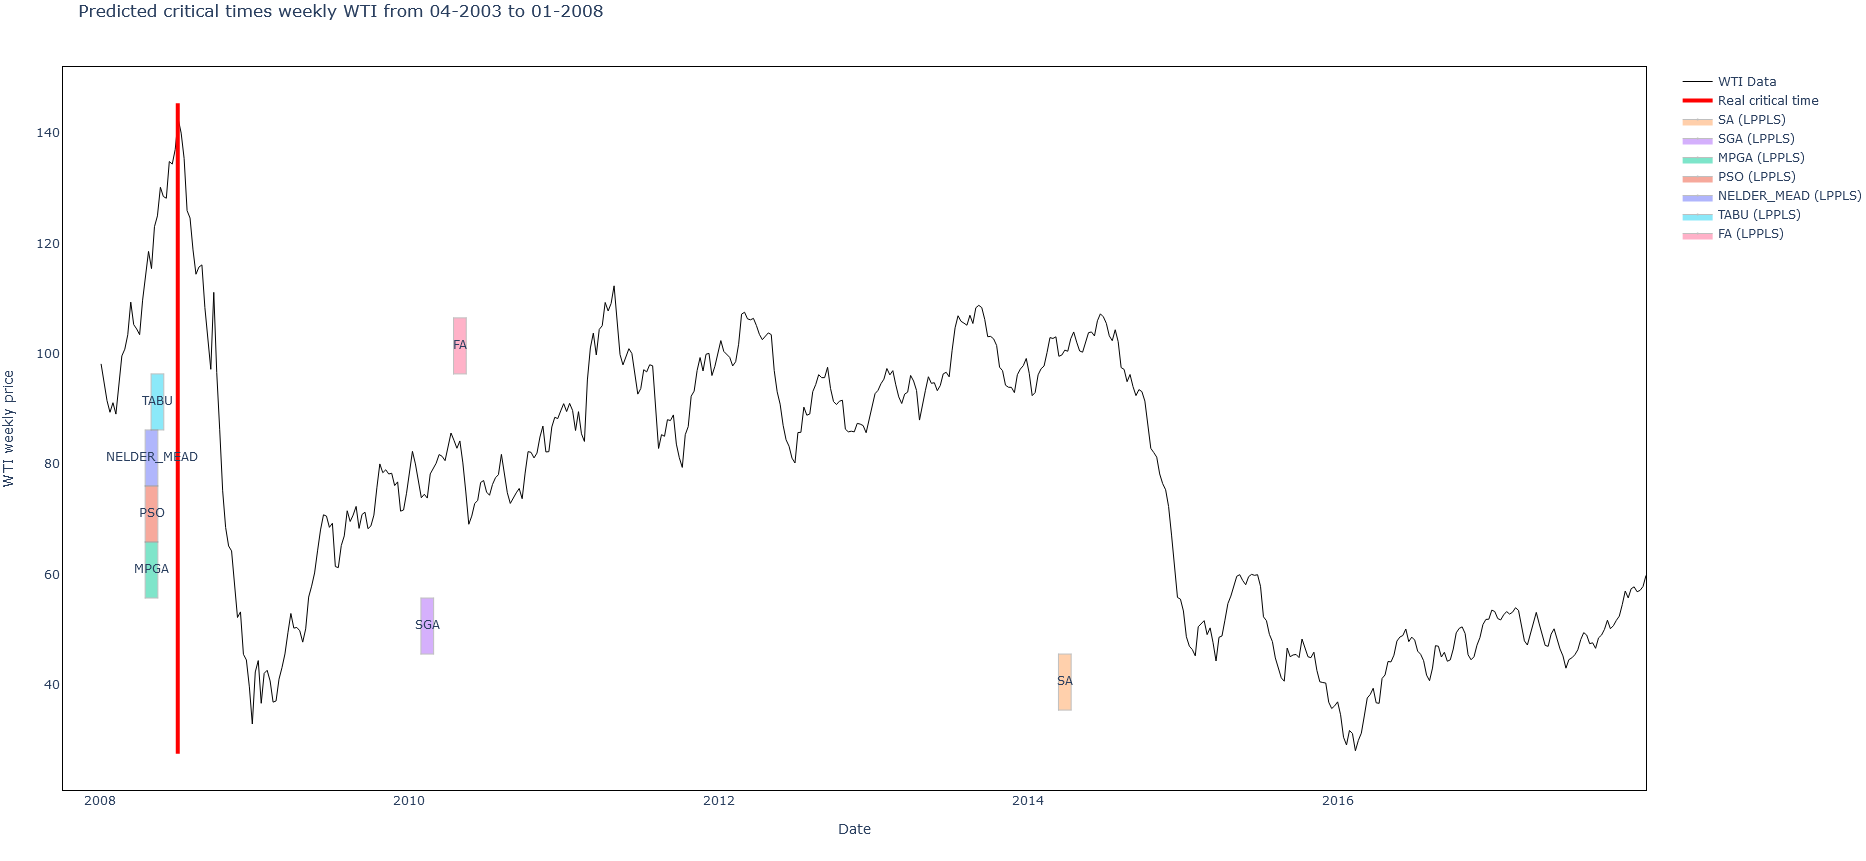
\includegraphics[width=\textwidth]{plot_overlead/weekly_WTI_1_LPPLS_all_price.png}
    \end{center}
\end{frame}

\begin{frame}{Comparison of Prediction Results (weekly)}
    \frametitle{Extensions : Results with LPPLS}
    \begin{center}
        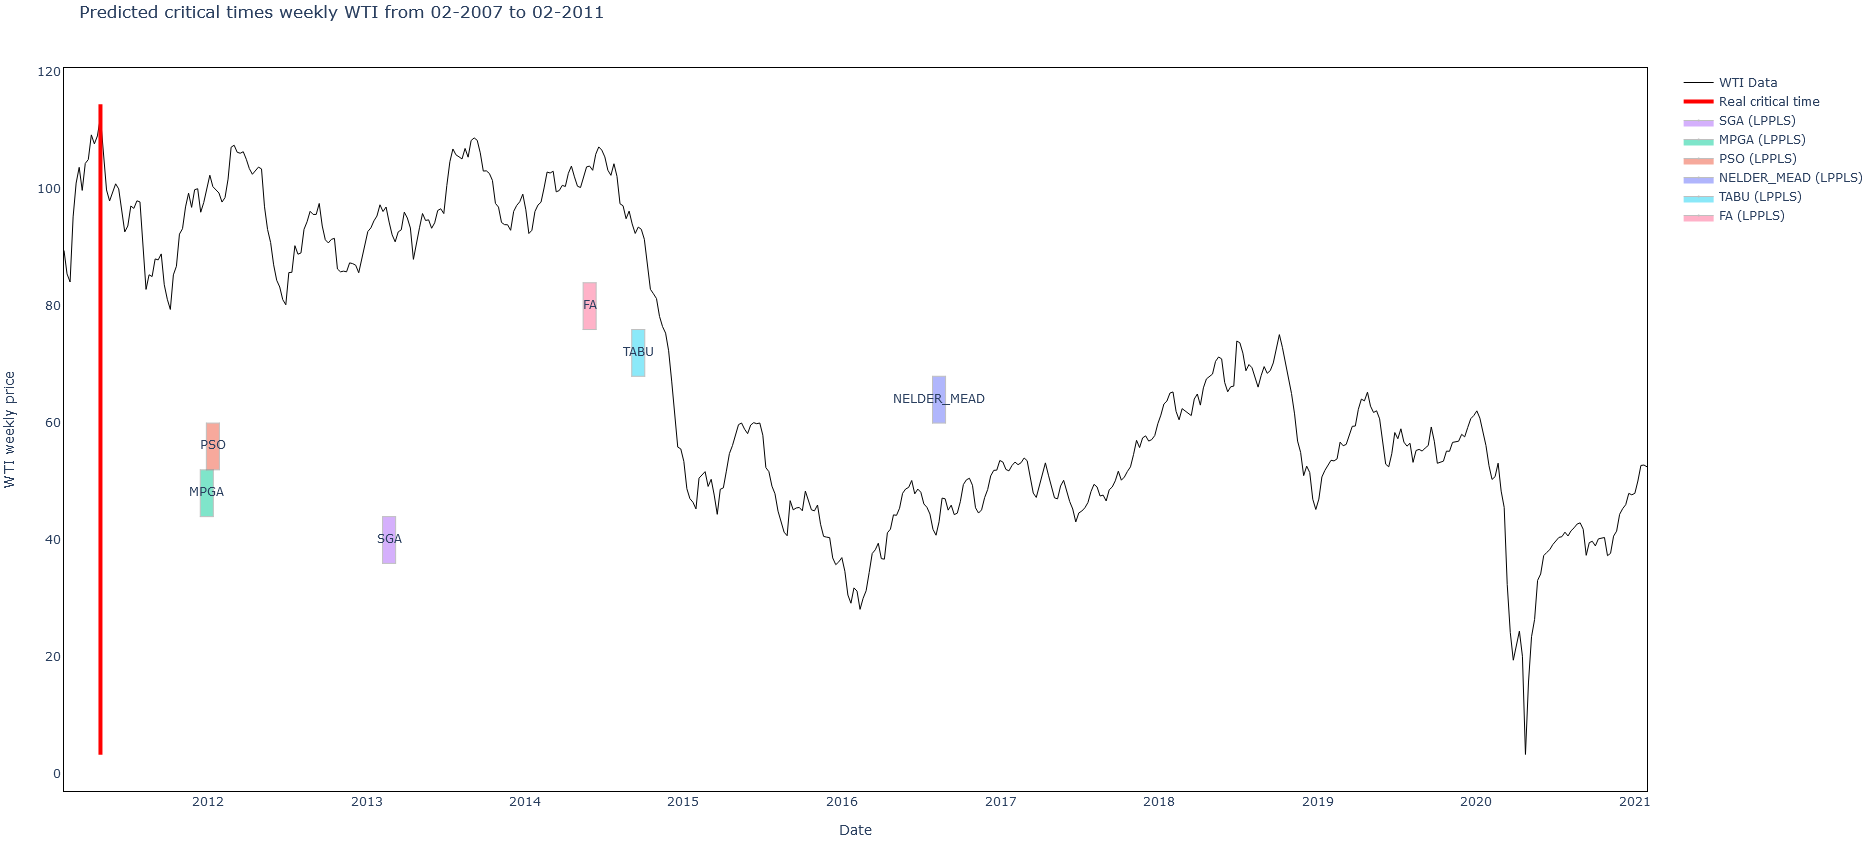
\includegraphics[width=\textwidth]{plot_overlead/weekly_WTI_2_LPPLS_all_price.png}
    \end{center}
\end{frame}

\begin{frame}{Comparison of Prediction Results (weekly)}
    \frametitle{Extensions : Results with LPPLS}
    \begin{center}
        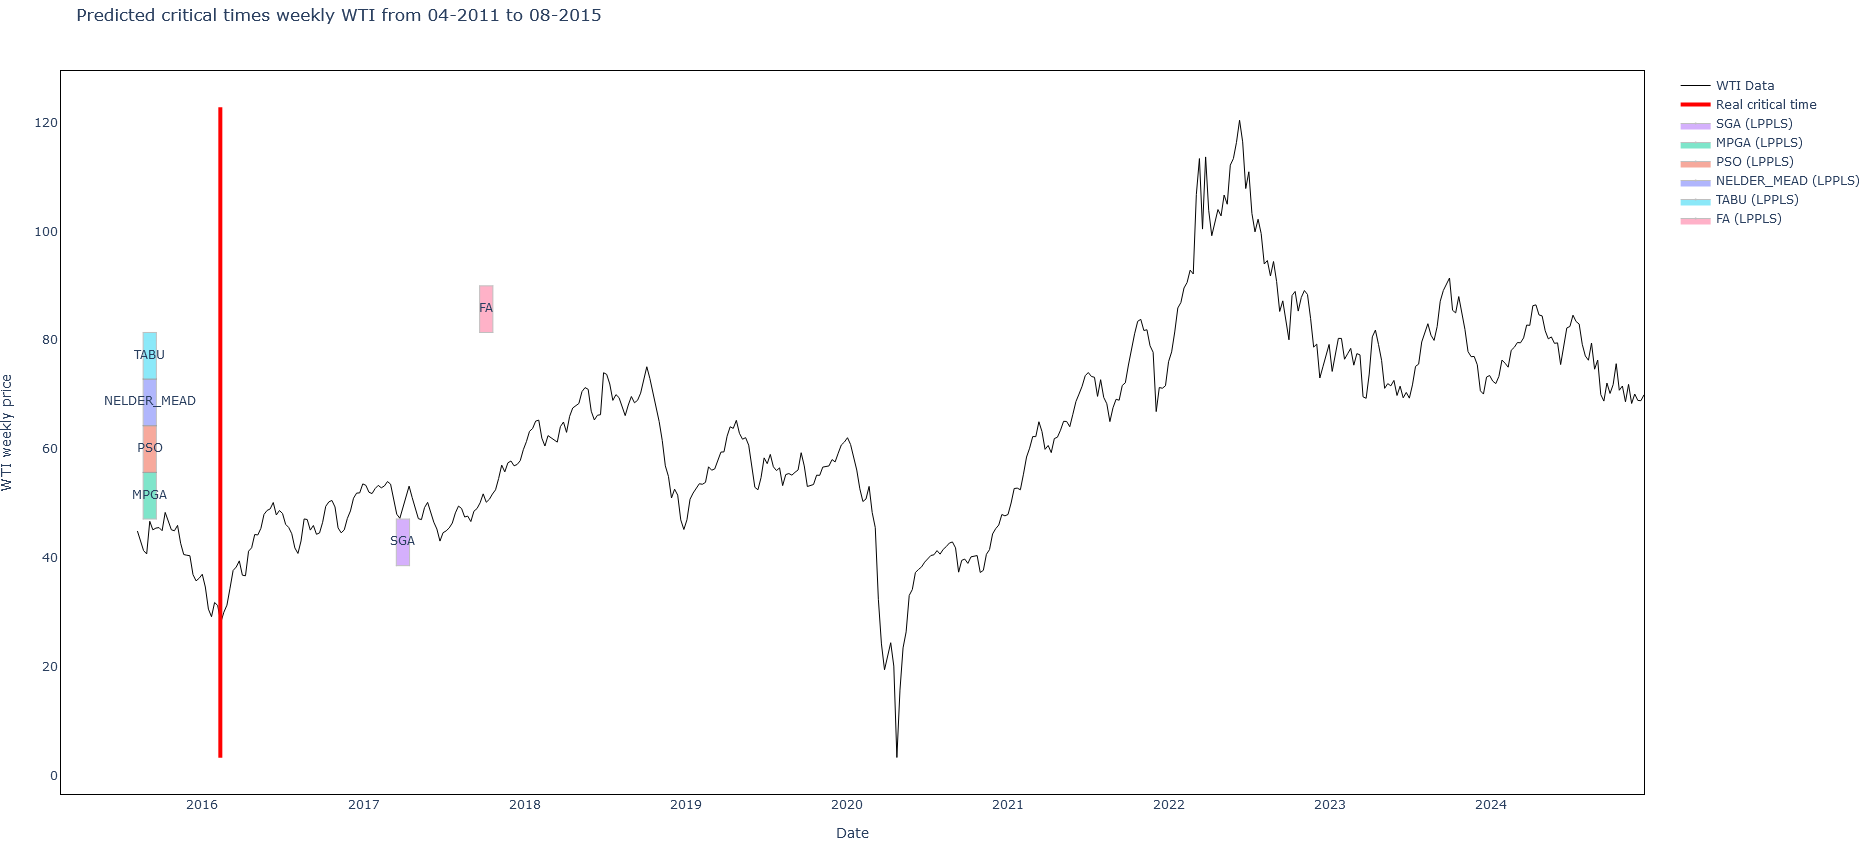
\includegraphics[width=\textwidth]{plot_overlead/weekly_WTI_3_LPPLS_all_price.png}
    \end{center}
\end{frame}

\begin{frame}
    \frametitle{Extensions : Turning point prediction on the S&P500}
    \begin{itemize}
        \item Graph(s) S&P500
        \begin{figure}[h]
        \includegraphics[width=8cm]{""}
        \end{figure}
    \end{itemize}
\end{frame}

\begin{frame}
    \frametitle{Extensions : Turning point prediction on the BTC}
    \begin{itemize}
        \item Graph(s) BTC
        \begin{figure}[h]
        \includegraphics[width=8cm]{""}
        \end{figure}
    \end{itemize}
\end{frame}

\begin{frame}
    \frametitle{Extensions : Turning point prediction on the EUR/USD}
    \begin{itemize}
        \item Graph(s) EUR/USD
        \begin{figure}[h]
        \includegraphics[width=8cm]{""}
        \end{figure}
    \end{itemize}
\end{frame}


\begin{frame}{Comparison of Prediction Results}
\frametitle{Extension}
\begin{table}[ht]
\centering
\caption{Comparison of prediction results of different heuristic algorithms.}
\resizebox{\textwidth}{!}{%
\begin{tabular}{|l|c|c|c|}
\hline
\textbf{Optimization Method} & \textbf{Turning Point 1} & \textbf{Turning Point 2} & \textbf{Turning Point 3} \\ \hline
Historical Turning Point     & \textbf{2008/07/03}      & \textbf{2011/04/29}      & \textbf{2016/02/11}      \\ \hline
30 days optimized by MPGA    & True (2008/06/29–2008/07/29) & True (2011/04/06–2011/05/06) & True (2016/02/10–2016/03/11) \\ \hline
4 weeks optimized by MPGA    & True (2008/06/20–2008/07/18) & True (2011/04/15–2011/05/13) & True (2016/01/15–2016/02/12) \\ \hline
30 days optimized by SGA     & True (2008/06/26–2008/07/26) & False (2011/09/04–2011/10/04) & False (2016/02/27–2016/03/28) \\ \hline
4 weeks optimized by SGA     & False (2008/07/11–2008/08/08) & False (2011/05/20–2011/06/17) & True (2016/02/05–2016/03/04) \\ \hline
30 days optimized by SA      & True (2008/06/26–2008/07/26) & True (2011/04/08–2011/05/08) & False (2016/02/19–2016/03/20) \\ \hline
4 weeks optimized by SA      & True (2008/06/27–2008/07/25) & False (2011/07/29–2011/08/26) & True (2016/01/15–2016/02/12) \\ \hline
30 days optimized by PSO     & False (2008/08/24–2008/09/23) & False (2011/06/17–2011/07/15) & False (2015/10/12–2015/11/11) \\ \hline
4 weeks optimized by PSO     & False (2008/07/11–2008/08/08) & False (2011/06/17–2011/07/15) & False (2015/08/21–2015/09/18) \\ \hline
30 days optimized by Nelder-Mead & True (2008/06/28–2008/07/28) & True (2011/04/10–2011/05/10) & False (2016/02/18–2016/03/19) \\ \hline
4 weeks optimized by Nelder-Mead & True (2008/06/25–2008/07/23) & True (2011/04/13–2011/05/13) & True (2016/01/16–2016/02/13) \\ \hline
30 days optimized by Tabu     & False (2008/07/02–2008/08/02) & False (2011/05/08–2011/06/07) & False (2016/02/23–2016/03/24) \\ \hline
4 weeks optimized by Tabu     & True (2008/06/29–2008/07/27) & False (2011/05/10–2011/06/09) & True (2016/02/03–2016/03/02) \\ \hline
30 days optimized by MCMC     & True (2008/06/30–2008/07/30) & True (2011/04/12–2011/05/12) & True (2016/02/17–2016/03/18) \\ \hline
4 weeks optimized by MCMC     & True (2008/06/22–2008/07/20) & True (2011/04/18–2011/05/18) & True (2016/01/14–2016/02/11) \\ \hline
\end{tabular}%
}
\end{table}
\end{frame}

\begin{frame}
    \frametitle{Window parameters finetuning}
    \begin{itemize}
        \item 2 years windows
        \begin{figure}[h]
        \includegraphics[width=8cm]{""}
        \end{figure}
    \end{itemize}
\end{frame}

\begin{frame}
    \frametitle{Window parameters finetuning}
    \begin{itemize}
        \item 1 years windows
        \begin{figure}[h]
        \includegraphics[width=8cm]{""}
        \end{figure}
    \end{itemize}
\end{frame}

\begin{frame}
    \frametitle{Window parameters finetuning}
    \begin{itemize}
        \item 6 years windows
        \begin{figure}[h]
        \includegraphics[width=8cm]{""}
        \end{figure}
    \end{itemize}
\end{frame}

\begin{frame}
    \frametitle{Window parameters finetuning}
    \begin{itemize}
        \item 2 month before the real tc
        \begin{figure}[h]
        \includegraphics[width=8cm]{""}
        \end{figure}
    \end{itemize}
\end{frame}

\begin{frame}
    \frametitle{Window parameters finetuning}
    \begin{itemize}
        \item 9 month before the real tc
        \begin{figure}[h]
        \includegraphics[width=8cm]{""}
        \end{figure}
    \end{itemize}
\end{frame}

\begin{frame}
\frametitle{Conclusion}
\begin{itemize}
    \item C'est à chier !
\end{itemize}
\end{frame}

\begin{frame}
    \frametitle{What's next ?}
    \begin{itemize}
        \item Insert graph with data of today
        \begin{figure}[h]
        \includegraphics[width=8cm]{""}
        \end{figure}
    \end{itemize}
\end{frame}

\end{document}